\documentclass[format=acmsmall, review=false, screen=true, anonymous=true, table]{acmart}

\usepackage{booktabs} % For formal tables
\usepackage{tabularx}
\usepackage{color, colortbl}
\usepackage{tabu}


\usepackage{tikz}
\usepackage{pgfplots}
\usepackage{textcomp}
\usepackage{siunitx}
%\pgfplotsset{compat=1.12}
%\usepackage{pgf-pie}
\usepackage{amsmath}
\usepackage[utf8]{inputenc}
\usepackage[russian,french,english]{babel}
\usepackage{wasysym}
\usepackage{comment}
\usepackage{subfigure}
\usepackage{indentfirst}


\usepackage[ruled]{algorithm2e} % For algorithms
\renewcommand{\algorithmcfname}{ALGORITHM}
\SetAlFnt{\small}
\SetAlCapFnt{\small}
\SetAlCapNameFnt{\small}
\SetAlCapHSkip{0pt}
\IncMargin{-\parindent}


% Metadata Information
\acmJournal{PACMHCI}
\acmVolume{9}
\acmNumber{4}
\acmArticle{39}
\acmYear{2010}
\acmMonth{3}
\copyrightyear{2009}
%\acmArticleSeq{9}

% Copyright
%\setcopyright{acmcopyright}
\setcopyright{acmlicensed}
%\setcopyright{rightsretained}
%\setcopyright{usgov}
%\setcopyright{usgovmixed}
%\setcopyright{cagov}
%\setcopyright{cagovmixed}

% DOI
\acmDOI{0000001.0000001}

% Paper history
\received{February 2007}
\received[revised]{March 2009}
\received[accepted]{June 2009}






\begin{document}
	%
	% paper title
	% can use linebreaks \\ within to get better formatting as desired
%	\title{Towards Bridging the Gap between Multilingual Q\&A Communities with Deep Learning \\
%		\large ---An Empirical Study of Russian Stack Overflow}


%\title[Multi-lingual Stack Overflow]{In Favor of or Against Multi-Lingual Q\&A Sites?: Exploring the Benefits and Concerns of Launching Multi-lingual Q\&A Sites}

\title[Multi-lingual Stack Overflow]{In Favor of or Against Multi-Lingual Q\&A Sites? Exploring the Evidences from User and Knowledge Perspectives}
	
\begin{abstract}
Many Q\&A sites initially run only in English, and then gradually release their multi-lingual variants to serve users who speak other languages.
The launch of such multi-lingual sites always leads to intense dispute about the pros and cons of multi-lingual sites.
Although all arguments and concerns sound reasonable, people can rarely provide solid evidence to convince each other.
In this paper, from users' comments about the launch of several non-English Stack Overflow sites, we first identify three major concerns including community split, knowledge needs and interests in other languages, and knowledge fragmentation and duplication.
To validate these three concerns, we conduct an evidence-based data analysis and comparison of user characteristics, tag usage and cross-site links between the Russian Stack Overflow and the English Stack Overflow on these three concerns.
Our study sheds the light on the existence value and risks of multi-lingual Q\&A sites.

       
\end{abstract}

\begin{comment}
Q\&A sites are emerging as a knowledge sharing and acquisition platform for different users, but most of them run in only one language (mostly English).
As not everyone can ask or answer questions in English, many Q\&A sites now begin to release their multi-lingual variants to serve users who speak other languages.
For example, in addition to the main English Stack Overflow, we now have Russian, Portuguese, Spanish and Japanese Stack Overflow.
The launch of such multi-lingual sites always leads to intense dispute about the pros and cons of multi-lingual sites.
Although all arguments and concerns sound reasonable, people can rarely provide solid evidence of their arguments and concerns to convince each other.
In this paper, from the users' comments about the launch of several non-English Stack Overflow sites, we first identify three major concerns including community split, knowledge needs and interests in other languages, and knowledge fragmentation and duplication.
We then conduct an evidence-based data analysis and comparison of user characteristics, tag usage and cross-site links between the Russian Stack Overflow and the English Stack Overflow on these three concerns.
Our results show that some special knowledge needs and interests in non-English languages warrant the value of multi-lingual Q\&A sites, and multi-lingual Q\&A sites do not result in community split.
However, knowledge fragmentation and duplication across multi-lingual sites is a valid concern.
Although manual cross-site linking can partially deal with this issue, the extent of knowledge fragmentation and duplication calls for automated cross-site linking and cross-site translation support.
%the concerns are not significant and validate the value of multi-lingual variants
\end{comment}

\begin{CCSXML}
	<ccs2012>
	<concept>
	<concept_id>10003120.10003130</concept_id>
	<concept_desc>Human-centered computing~Collaborative and social computing</concept_desc>
	<concept_significance>300</concept_significance>
	</concept>
	</ccs2012>
\end{CCSXML}


%\ccsdesc[500]{Applied computing~Text editing}
\ccsdesc[300]{Human-centered computing~Collaborative and social computing}

%
% End generated code
%


\keywords{Multi-lingual Q\&A Site; Stack Overflow; Community Split; Knowledge Needs and Interests; Knowledge Fragmentation and Duplication; Cross-Lingual Retrieval}

% make the title area
\maketitle
	
	
	% For peer review papers, you can put extra information on the cover
	% page as needed:
	% \ifCLASSOPTIONpeerreview
	% \begin{center} \bfseries EDICS Category: 3-BBND \end{center}
	% \fi
	%
	% For peerreview papers, this IEEEtran command inserts a page break and
	% creates the second title. It will be ignored for other modes.
	
	\section{Introduction}
A community question and answer (Q\&A) website provides a collaborative information seeking platform for users to ask and answer questions.
The accumulated questions and answers over time create a crowdsourced knowledge base which can benefit many people (in addition to the question askers themselves) who have similar questions.
Recent years have witnessed the unprecedented development of Q\&A websites such as Stack Exchange and Quora. 

\begin{comment}
\begin{figure}
	\centering
	\subfigure[Spanish Stack Overflow]{%
		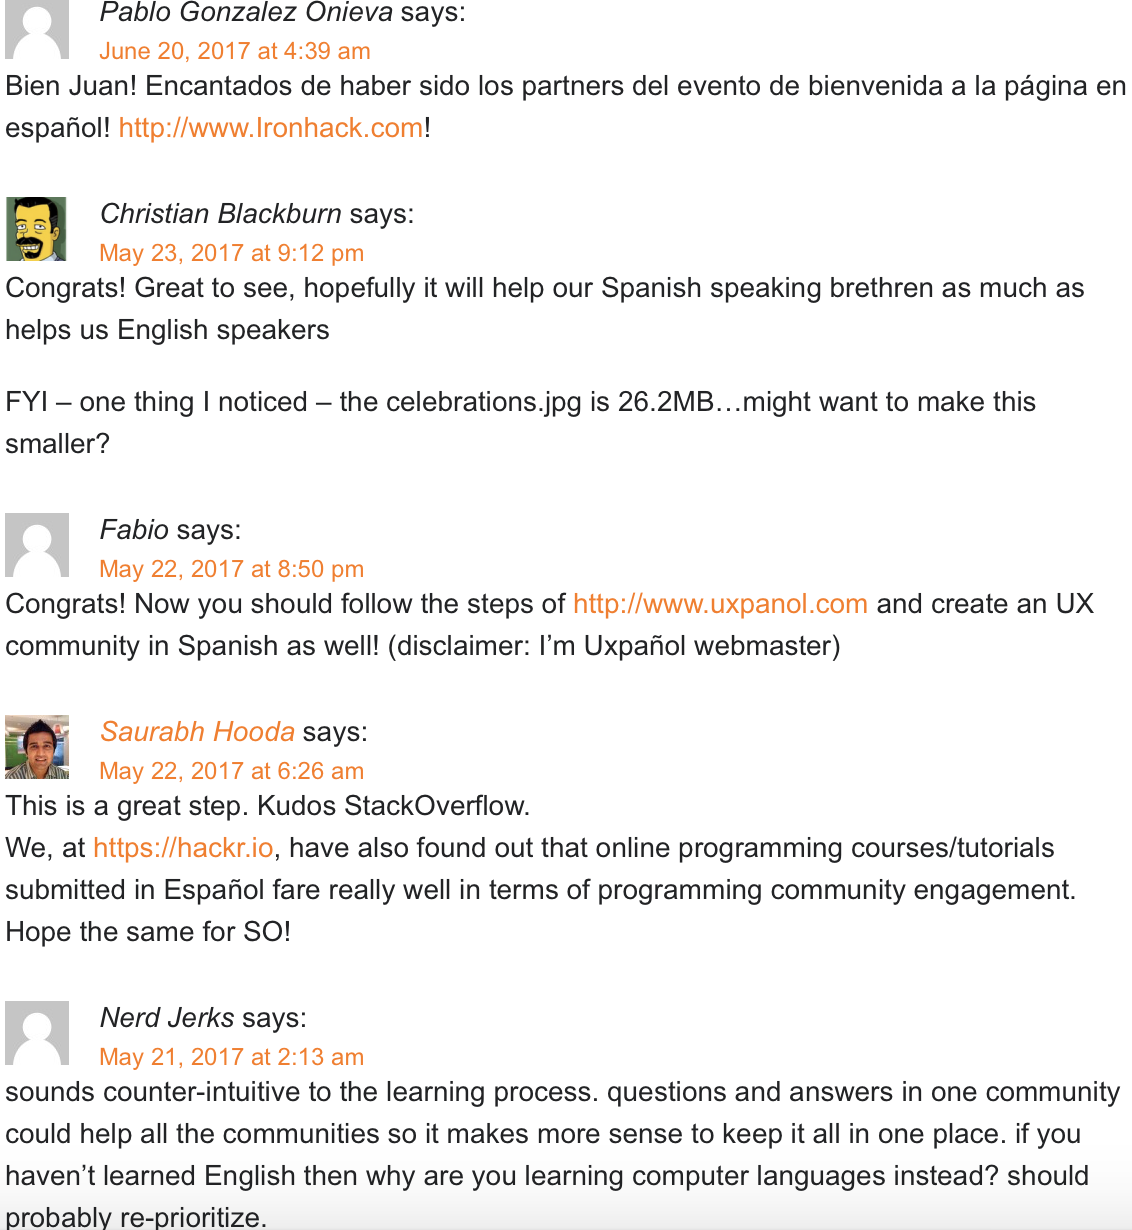
\includegraphics[width=0.42\textwidth]{figures/SOcomment.png}
		\label{fig:SOcomment}
	}
	\hfill
	\subfigure[Spanish Quora \textcolor{red}{suggest not to use Quora. Consider using a post example on Meta Stack Overflow}]{%
		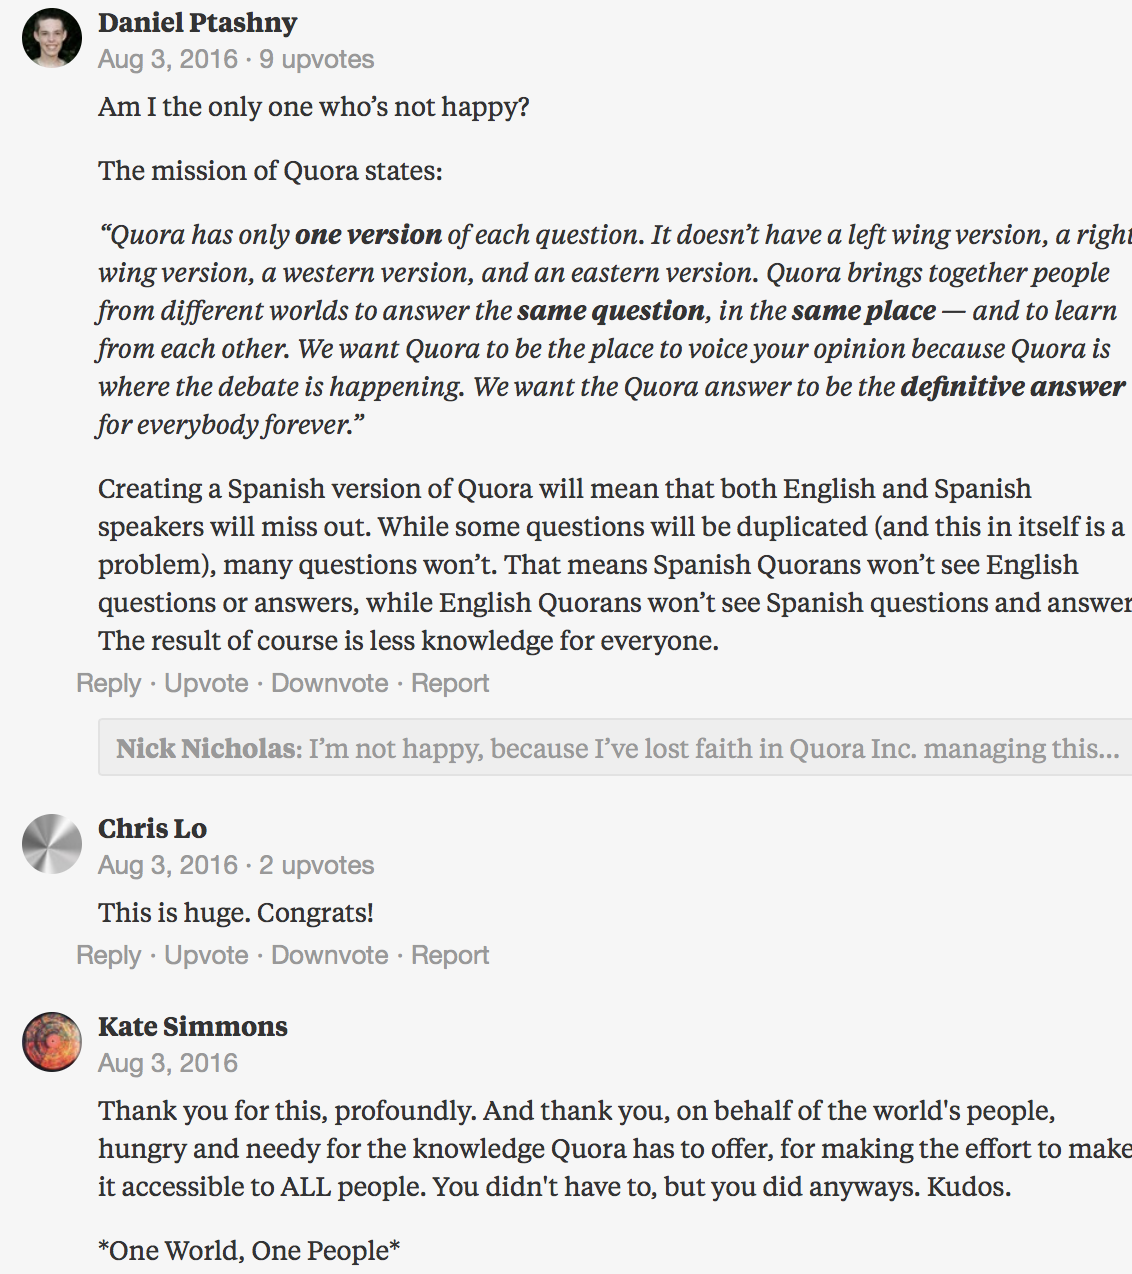
\includegraphics[width=0.42\textwidth]{figures/QuoraComent.png}
		\label{fig:QuoraComment}
	}
	\caption{Example user comments and discussions on the launching of multi-lingual Stack Overflow sites
		\textcolor{red}{
			1) I say not to show Quora example here. Quora is for general domain which may have completely different phenomena from Stack Overflow. It is very likely that our findings on Stack Overflow cannot be extended to Quora. And this will invite questions why not study both Stack Overflow and Quora and contrast them to gain even deeper insights. I say if we really want to discuss Quora, mentioning it only in the Discussion section as future work.
			2) Still use two examples. One from the comments left on the announcement. The other from the separate post discussion. No need to use screenshots. Very hard to read. Instead, use a table or so to quote the comments. 
			3) Organize the comments into three parts: community split, knowledge interests, knowledge fragmentation/duplication. For each part, list one or two supporting comments and one or two against comments. Highlight key phrases in the comments to attract the readers' attention. 
		}
	}
	\label{fig:userComments}
\end{figure}
	
\end{comment}
  
\begin{figure}
	\centering
	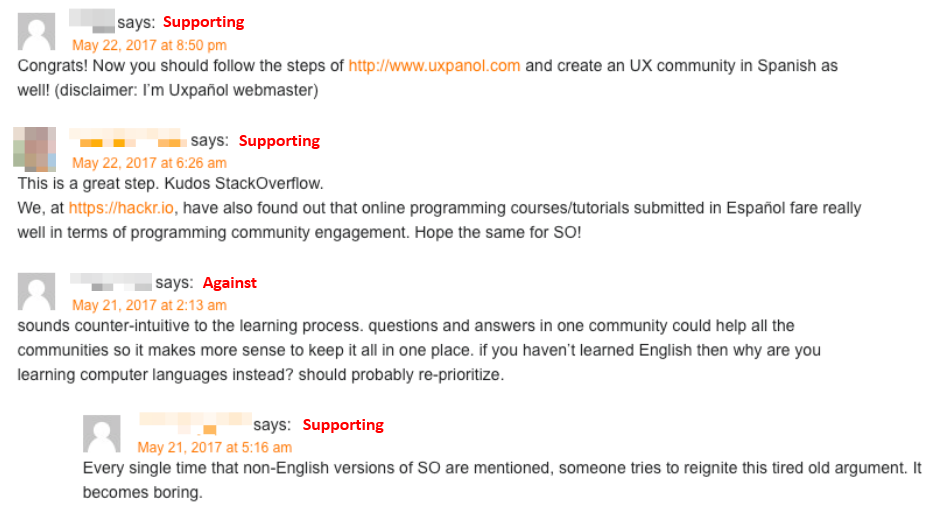
\includegraphics[width = 0.95\textwidth]{figures/SpanishSO.png}
	\caption{Example user comments and discussions on the launching of Spanish Stack Overflow site~\cite{web:SOspanish}}
	\centering
	\label{fig:userComments}
\end{figure}  

Originally, most of the Q\&A sites run in one language (mostly English).
However, %English is only one of \textcolor{red}{xxx} languages in the world.
for those who do not speak English or do not use English as their working language, they cannot directly access such English Q\&A sites due to the language gap.
%However, this non-English population is a big potential market for a successful English Q\&A site to extend its business.
To make the site available for non-English population, many Q\&A sites begin to release their multi-lingual variants to serve users who speak other languages.
Note that a multi-lingual variant of a Q\&A site is neither the translation version of the original English site, nor the original site with language localisation features.
Instead, it is a totally new site for a non-English language but adopts the same policies, practices and supports the same look and feel and user experience as the original English site.
For example, there are Russian, Japanese, Portuguese, Spanish Stack Overflow\footnote{\url{https://stackoverflow.blog}}, and French, Spanish, Japanese, German, Italian Quora\footnote{\url{https://blog.quora.com}}.
Despite these benefits, the decisions of launching some multi-lingual variants of the original English site always cause intense dispute about the pros and cons of multi-lingual variant sites among users.
This is evident from the supporting- or against-comments that users left on the announcement of the new multi-lingual sites~\cite{web:SOjapanese, web:SOportugese1, web:SOportugese2, web:SOrussian, web:SOspanish}.
Users also created some posts on Meta Stack Exchange and Meta Stack Overflow to discuss the points in favour of or against multi-lingual sites~\cite{web:SOdiscussion1, web:SOdiscussion2, web:SOdiscussion3, web:SOdiscussion4, web:SOdiscussion5, web:SOdiscussion6, web:QuoraDiscussion}.

Fig.~\ref{fig:userComments} presents one typical example of such dispute about the multi-lingual Stack Overflow sites.
We conduct a formative study in which we crawl all the user comments on the launch of multi-lingual Stack Overflow sites.
Three major concerns emerge from our analysis: 
\textit{community split}, \textit{knowledge needs and interests in English and other languages}, and \textit{knowledge fragmentation and duplication}.
On the one hand, users who are against the multi-lingual sites are worried about: this would cause the community split across different sites, whether there are enough needs and interests in computer programming knowledge in other languages, and knowledge fragmentation and duplication across different sites would become a serious issue to deal with.
On the other hand, users who support the multi-lingual sites argue that: the multi-lingual sites could involve more non-English-speaking users in the community, there are different knowledge needs and even unique knowledge interests for non-English-speaking users, and knowledge duplication may not be a bad thing as long as good questions and answers in one language could be referenced or translated in another language.
  
People use different examples, reasons, arguments to defend their opinions, but they can rarely provide solid evidences to convince others, and thus the same dispute repeats once another multi-lingual site is launched.
Some users point out the needs for more evidence-based analysis of multi-lingual sites, rather than just conjecturing what would or would not happen.
For example, this user suggests in his post~\cite{web:SOdiscussion1} that ``\textit{We need to see charts of activity by country to gauge how many people this would bleed away from the main site. My guess is, it's a lot more than you'd expect}''.
With the launch of multi-lingual sites and the data accumulated on these sites over time, it becomes feasible for evidence-based analysis and comparison between the multi-lingual sites and the original English site, which will give us insights into the value of multi-lingual sites, their impacts on the original English sites, and the necessary tools to support the multi-lingual sites.

In this paper, we conduct such an evidence-based data analysis and comparison between the Russian Stack Overflow (RSO) and the English Stack Overflow (ESO).
We choose Stack Overflow as the subject site because it is the most successful and popular Q\&A site for computer programming and it provides up-to-date data dump of the entire site information for public use and research.
We choose Russian Stack Overflow because it is the largest multi-lingual Stack Overflow variant with sufficient users and posts for the comparative study.
Inspired by the three major concerns we identify in our formative study of the user comments on the launch of multi-lingual Stack Overflow sites, we focus our analysis on three points.
First, we study the risk of community split from the user perspective by analyzing user registration, user reputation score, and user posting behavior on RSO and ESO.
Second, we study the knowledge needs and interests in English and Russian from the tag perspective by analyzing tag frequency correlation and tag uniqueness between RSO and ESO.
Third, we study the knowledge fragmentation and duplication issue from the cross-site linking perspective by analyzing existing manual cross-site links by users and potential cross-site links that users are not aware of.

Our results show that some special knowledge needs and interests in non-English languages warrant the value of multi-lingual Q\&A sites, and multi-lingual Q\&A sites do not result in community split.
However, knowledge fragmentation and duplication across multi-lingual sites is a valid concern.
Although manual cross-site linking can partially deal with this issue, the extent of knowledge fragmentation and duplication calls for automated cross-site linking and cross-site translation support.

%Therefore, in this work, we carry out data-driven empirical study to check the main pros and cons quantitatively.
    
%We first summarise users' opinions from their comments under the announcement of multi-lingual new sites in Stack Overflow blogs.
%The pros and cons are concluded as the motivation of this work.
%We especially take the Stack Overflow and Russian Stack Overflow as the case study to investigate the mutual influence between two sites.
%We then analyse their relationships from different aspects such as 
%.....

The main contributions of this paper are listed below:	
\begin{itemize}
	\item This work is the first quantitative study of the phenomena and effects of multi-lingual Q\&A sites. 
	It provides evidences to validate the existence value of multi-lingual Q\&A sites, the risk of community split, and the issue of knowledge fragmentation and duplication. 
	%variants and validates the concerns of the community split and duplicate content in the new site, but the effects are rather small. 
	\item Our study identifies a new problem for the development of multi-lingual Q\&A sites, i.e., manual cross-site linking is not sufficient for bridging the knowledge across multi-lingual sites. We provide a cross-site retrieval method which has potential to tackle this problem. 
	%\textcolor{red}{CCY: I think we need to tune down for our cross-site retrieval method.}
	\item Inspired by our findings, we envision cross-site retrieval and cross-site translation techniques to better support multi-lingual Q\&A sites, and identify key challenges in developing such techniques.
	%based on our discovery to assist new sites. The tool is needed for helping locate reference of old questions in the main site, and translate accepted answer to target language.
\end{itemize}

\begin{comment}
	
	Stack Overflow is a platform with millions of users and huge amount of content. Table 1 presents the statistics of users, posts and comment Stack Overflow main site and other lingual sites. As shown, the number of users as well as the amount of posts and comments in the English main site are much higher than the other multilingual sites. Also, there are only 50\% to 60\% of the lingual variant users who also use the Stack Overflow main site at the same time. This indicates that a considerable sum of users only use the lingual variant site which means they may ask or answer some questions already existing on the main site.
	
   	To get more potential users over the world and extend the current business model, setting up the new multilingual sites based on Tehran current English main site has been a very popular strategy for the English Q\&A websites. So does Stack Overflow. Since Ethe coding language are developed and based on the English Stack Overflow, a codeing Q\&A website, were originally developed in English and it has become the msot popular coding Q\&A website in the world. It also starts to run the multilingual sites aiming to different programer communities in other languages. Because the native language is much more attractive for the native speakers, and the long term goal of Stack Exchange Network is to be a great and planetary resource for worldwide citizens no matter what language they speak [8].
\end{comment}
   	
   	
   	%To get more potential users over the world and extend the current business model, setting up the new multilingual sites based on the current English main site has been a very popular strategy for the English Q\&A  websites. So does Stack Overflow. Since the coding language are developed and based on the English, Stack  Overflow, a coding Q\&A website, were originally developed in English and it has become the most popular coding  Q\&A website in the world. It also starts to run the multilingual sites aiming to different programmer communities in other languages. Because the native language is much more attractive for the native speakers, and the long term goal of Stack Exchange Network is to be a great and planetary resource for worldwide citizens no matter what language they speak [8].
   
\begin{comment}	
   	Therefore, it is meaningful if a clear answer can be found when websites and communities keep developing their multilingual variants, and more contributions is supposed to be made to bridge the lingual gap for all users who are interested in some content on the website writing in other language. It is highly believed that humans are accustomed to a more familiar environment [24], especially lingual environment. Although some people learn a second language, when the question is related to a domain-specific topic with a lot of professional words it is also very hard for them to search, understand or express their thoughts clearly. 
\par
	The active level of a community is determined by many factors, and the most important ones are users and content. Comparing the statistics in Table 1, it is clear that the number of user in Stack Overflow main site is around 90 times that of Russian Stack Overflow, and the content in the main site is also much more than the other multilingual sites which means the gap of their resources may be enormous. To clearly identity and quantitatively analysis this difference,  an empirical study on the users and content between the Stack Overflow main site and Russian Stack Overflow has been conducted. The main research object is locked on the Russian Stack Overflow besides the main site, since it has the top number of users and top amount of posts as well as comments than other multilingual variants. 
	\par
	
		There are several interesting cases on the sites of Stack Overflow, which are presented in Figure 1. The sub-figure a) shows a very common phenomenon that users from the other lingual sub-site of Stack Overflow like the Russian variant often cannot find satisfying and high-quality answers on other lingual Stack Overflow sites, which need to be defined as {\bf sub-sites}, for some reasons, while the main site can always assists them with the solutions. The sub-figure b) is a answer posted on Russian Stack Overflow, which means, in English, there are some previous solutions on the Stack Overflow English main site for this specific Russian question. 
\par
	Imagine that a Russian speaker who cannot speak English fail to find a good answer to his or her question. Meanwhile, the reply to his post is quite slow because the number of users on Russian Stack Overflow is small. For this problem, our cross-lingual question retrieval model can efficiently deal with the lingual gap problem and recommend useful resources across different languages. A key benefit of this approach is the non-English speakers can efficiently utilize the huge knowledge base from the dominant English community.
\end{comment}   	
	


	
\section{Related Work}
There are many crowd-source knowledge-sharing websites in the world such as Q\&A websites (like Quora and Stack Overflow) and Wikipedia.
Although most of them begin with only English, the support of other languages has beed added later to make the site more accessible to non-English speakers.
There is a growing field of research on multilingual Wikipedia.
The general consensus on multilingual Wikipedia is that while English (the largest language edition) has a content advantage, each language edition has a great deal of unique information that is not available in other language editions~\cite{filatova2009multilingual, hecht2010tower}.
%, and most other information exists in only a few language editions
In contrast, the launch of Q\&A sites in different languages has caused intense dispute, no matter for Stack Overflow~\cite{web:SOdiscussion1, web:SOdiscussion2} or Quora~\cite{web:QuoraDiscussion}. 
Albeit bitter debate, it does not attract much attention from researchers to investigate multi-lingual Q\&A sites.
Our work attempts to fill in such a gap by carrying out a quantitative empirical study of multi-lingual Stack Overflow sites to explore the evidences in favor of or against multi-lingual Q\&A sites.

As Wikipedia now owns more than 200 different editions for different languages, it encourages users to translate articles from the English Wikipedia into other languages with official guideline~\cite{web:WikipediaMultiLingual}.
However, as sorely manual translation is time-consuming and labor-extensive, many researchers propose methods to help cross-lingual linking~\cite{wang2012cross, wang2014cross, wulczyn2016growing}, or aid humans in propagating information from one Wikipedia (typically English) to another (typically a language edition with a small number of articles) by using machine translation~\cite{adar2009information, kumaran2010wikibabel, bao2012omnipedia}.

There are also some works supporting multi-lingual retrieval specifically in Stack Overflow~\cite{xu2016domain, chen2016learning}.
To find related questions in Stack Overflow, Xu et al.~\cite{xu2016domain} translated the Chinese query into English with online translation service, while Chen et al.~\cite{chen2016learning} mapped both Chinese queries and English questions into the same vector space for cross-lingual retrieval.
Different from their works, we mainly focus on the validation of users' concerns of multi-lingual Q\&A sites including community split, knowledge interests and needs in other languages, and also knowledge fragmentation and duplication.
We discuss the potential of extending our method in Section \ref{sec:crossLinking} for linking posts across multi-lingual sites, and also the feasibility of customising the state-of-the-art machine translation to help translate domain-specific posts in Section~\ref{sec:crossTranslation}. 

\begin{comment}
%\textcolor{red}{Some related work about multi-lingual Quora, Wikipedia...}
\textcolor{orange}{Asking questions in natural language within a certain community and obtaining the exact domain-specific answers make the Q\&A websites becoming more and more powerful on information retrieval as well as generaing the searchable and valuable informaion for the community. Several reseaches shows that comparing with the general search enginesa a well-organized and highly active Q\&A community could be more useful for retrievaling relevant domain-specific information to the users who have such a need~\cite{dominique2006qabetter,Daniel2006adapting,Anne2006evaluation}. Thus, in the last decade, many crowd-source knowledge-sharing websites in the world have developed very fast, such as Q\&A websites (like Quora and Stack Overflow) and Wikipedia.}
Although most of them begin with only English, the support of other languages has been added later to make the site more accessible to non-English speakers.
There is a growing field of research on multilingual Wikipedia.
The general consensus on multilingual Wikipedia is that while English (the largest language edition) has a content advantage, each language edition has a great deal of unique information not available in other language editions, and most other information exists in only a few language editions~\cite{filatova2009multilingual, hecht2010tower}.
\textcolor{orange}{However, the multilingual and transliongual Q\&A systems is much more complex and difficult to run than multilingual Wikipedia.}
\textcolor{orange}{The research conducted by Teruko et al~\cite{Teruko2006keyword}. addresses that the translation quality on the domain-specific keywords has significant influence to the performance of a cross-lingual Q\&A system developed from a monolingual one.}
\textcolor{orange}{The research conducted by Soojung Kim et al~\cite{Soojung2008}. indicates that in a social Q\&A environment people share not only the specific information but also the subjective opinions and suggestions with a set of common criteria frequently used in people's relevance judgment regardless of the contexts. This could lead to the difficulty of yielding the most helpful answers for the asked questions on a Q\&A website.}
\textcolor{orange}{There is also a research conducted by E.W.D.Whittaker et al.~\cite{EWD2006mono} addressing that the difficulty of building a cross-lingual system based on the English language database is the lack of the corresponding NLP tools in the target language. They addressed that the huge diversity on the grammar, syntax and semantics of different languages makes it very difficult to develop a multilingual NLP system. The global development plan of WordNet is an example which still only cover a relatively small number of languages after being ported to other languages rather than English. This lead to the gap between language-specific database and system.}
However, few similar research works has been extended to Q\&A sites.
Our work is trying to fill in such gap by carrying out a quantitative empirical study in Stack Overflow to investigate the effects of multi-lingual variants to their main site.
As Wikipedia now owns more than 200 different editions for different languages, many research are helping cross-lingual linking~\cite{wang2012cross, wang2014cross, wulczyn2016growing}, or aid humans in propagating information from one Wikipedia (typically English) to another (typically a language edition with a small number of articles) by using machine translation~\cite{adar2009information, kumaran2010wikibabel, bao2012omnipedia}.
There are also some works supporting multi-lingual retrieval in Stack Overflow~\cite{xu2016domain, chen2016learning}.
In this work, we mainly focus on the validation of users' concerns of multi-lingual variants, but we also discuss the potential of extending our method in Section \textcolor{red}{??} for linking posts in multi-lingual site.
We also discuss the feasibility of customising the state-of-the-art machine translation to help translate the accepted answers to the new sites. 

	
\end{comment}



\begin{comment}
This section introduces the related work of our paper. 
We mainly present works about and the multi-lingual retrieval, especially in software engineering, then deep learning techniques in software engineering.
\subsection{Q\&A Websites with Multiple Languages}
With the development of internet, Q\&A websites have become vital knowledge base for users, especially the technical sites like Stack Overflow for the programmers. Information retrieval is a good approach to assist people utilizing the resource on these platforms. Researchers classify this topic into two main parts, which are document retrieval and code retrieval. For our study, we mainly focus on the document retrieval part. So far, a lot of heuristic research has been done in this particular area. They divide the relationship with two different questions into four types, which are Duplicate, Direct Link, Indirect Link and isolated, and formulate a multi-class classification approach, which is considered as a good future work for our approach.
\par



\subsection{Multi-lingual Retrieval}
There are a lot of deep learning applications in the software engineering field and have made excellent results. Some effective tools like {\bf word2vec} and {\bf GloVe} [26]have been developed for learning words representation, which assists the researchers efficiently process the word embedding tasks. In our approach, we adopt GloVe to process the learning word representation tasks because it can achieve a high level of accuracy in a shorter time with using the negative samples.
\par
The semantic similarity is always a most attractive topic in the neuro-linguistic programming area. A lot of good approaches have been developed on this topic. For example, the model for detecting the question similarity [27] and the model for detecting relevant tweets [28]. These existing well-designed models formulate the problem into a binary classification problem, which is duplicate and non-duplicate.
It is necessary to note that there are a number of experts manually mark the highly similar questions as duplicate ones on the Stack Exchange Site. Considering the data structure that we can mine, these binary classification approaches are highly responsive to our scenario and worthy for us to learn.
\par
A highly heuristic work has been carried out recently. As mentioned above, we generate 0.3 million of duplicate pairs for training the deep learning model. Somehow, the amount of training data might be small. Using post body as the corpus to pre-train an RCNN model for generating plenty of titles [29] can solve the problem with insufficient training data. We consider this approach as a good supplement for our model.

There are also some multi-lingual retrieval works specifically in software engineering.
A CNN cross-lingual domain specific model explored some doable methods to overcome the lingual gap [20]. 
Another excellent work has been carried out on cross-lingual issues in software engineering. The cross-lingual bug localization[25] and the domain-specific multi-classification approach [18] are both focusing on the cross-lingual problem between English and Chinese.
Compared with their works, we 


\subsection{Deep Learning for Software Engineering}
There are a lot of deep learning applications in the software engineering field and have made excellent results. Some effective tools like {\bf word2vec} and {\bf GloVe} have been developed for learning words representation, which assists the researchers efficiently process the word embedding tasks. In our approach, we adopt GloVe to process the learning word representation tasks because it can achieve a high level of accuracy in a shorter time with using the negative samples.
\par
The semantic similarity is always a most attractive topic in the neuro-linguistic programming area. A lot of good approaches have been developed on this topic. For example, the model for detecting the question similarity [9] and the model for detecting relevant tweets [10]. These existing well-designed models formulate the problem into a binary classification problem, which is duplicate and non-duplicate.
It is necessary to note that there are a number of experts manually mark the highly similar questions as duplicate ones on the Stack Exchange Site. Considering the data structure that we can mine, these binary classification approaches are highly responsive to our scenario and worthy for us to learn.
\par
A highly heuristic work has been carried out recently. As mentioned above, we generate 0.3 million of duplicate pairs for training the deep learning model. Somehow, the amount of training data might be small. Using post body as the corpus to pre-train an RCNN model for generating plenty of titles [29] can solve the problem with insufficient training data. We consider this approach as a good supplement for our model.

\end{comment}
\begin{comment}
		\subsection{Recommender System}
	Generally, recommender system generates the recommendation in two ways, one is collaborative and content-based filtering and the other is personality-based approach [6]. The measure of a recommender system is the efficiency and accuracy. On the Q\&A websites, there are already exist many recommendation engines, users can easily input the search keyword and the searching engine will automatically return a list of answers. However, this form of recommender system can only utilize a large number of resource, it is not the best approach in the other aspects. \par
	
	There are some studies carried out in this area with different aims like recommending relative papers or programming analogical libraries [7, 8]. The later one is highly heuristic because the analogical libraries cannot be recommended by the current search engine, the traditional way is manually searching for the answer on the Internet. While using Deep Learning method can train the model with the keywords and the specific library, this approach can overcome the gap between the textual and programming language. \par
	
	According to the “Enrichment Effect” on the Q\&A website that means a few number of hotly debated posts can easily get a large number of answers and comments, while the areas that are not too hot will hardly receive some valuable feedbacks. We are also facing the same challenge. For the small multilingual subsites, a small number of users and a narrow knowledge base sometimes cannot support an efficient information exchange process. Therefore, our approach needs to keep in a high level of performance in this situation to beat the traditional recommender system.
	
	
	\subsection{Letter Level}
	From the literacy review, we found some excellent work that has been done in the more bottom level than the semantic level, such as the word level and letter level research [11]. Y. Shen, X. He, J. Gao, L. Deng, and G. Mesnil used the word-n-gram and letter-trigram model to build up a latent semantic model with pretty good results. The difference between the letter-trigram embedding with traditional word embedding is that every single word in the corpus needs to generate some letter trigrams. The letter trigrams represent all the sentences in the low dimensional vector space and then calculate the similarity between them. This method works very well in the letter and word levels, but the difficulty is that there is no well-developed letter trigram base. Nevertheless, this approach is also implemented. We trained this approach and compare the results with those of our DSSM approach in the experiment section. We generate a letter-trigram base from the corpus that we mined from Stack Overflow. Although the amount of letter trigram is not as great as we thought at first, we still apply the trigram base for letter embedding. 
	\par
	This research [11] is also a good enlightenment for the future improvement of our approach because the semantic similarity calculation can also benefit from both letter and word levels. A better result would be made in the future if we can combine these techniques. 
	
	\subsection{ Information Retrieval and Semantic Similarity}
	There is also some heuristic works in this field. Especially, some research on the Dual-language information retrieval is very remarkable. The CNN cross-lingual Domain-specific model explored some doable methods to overcome the lingual gap[12].  On the other hand, the semantic similarity is always a most attractive topic in the neuro-linguistic programming area. Also, some powerful libraries like word2vec and GloVe are developed in recent years, which help the researchers efficiently handling the word embedding process. In our approach, we need to use GloVe because it can achieve a high level of accuracy in a shorter time with using the negative samples.
	\par
	
	Some research has been already made in detecting similar questions~\cite{chen2016learning} and relevant tweets[10]. These existing well-designed works have formulated the problem in a binary prediction problem, which is duplicate and non-duplicate. In Stack Overflow community, there are always some people marking the posts with different content as duplicate posts because they are actually the same question on the semantic level. The duplicate attribute can distinguish all the existing posts into two groups, which are also duplicate post and non-duplicate posts. These existing works highly correspond to our scenarios.
	content...
\end{comment}	
	\section{Formative Study of the Concerns about Multi-Lingual Stack Overflow Sites}
In Stack Overflow, questions, answers and comments are required to be written in English~\cite{web:SOenligsh}.
As not all developers can ask or answer questions in English, the founders of English Stack Overflow would like to explore the feasibility to launch multi-lingual Stack Overflow, i.e., Stack Overflow in other languages.
After the beta development process\footnote{\url{https://stackoverflow.com/help/whats-beta}}, several non-English Stack Overflow sites have been launched including Russian, Portuguese, Spanish, and Japanese one.
Each time a new non-English Stack Overflow site has been launched, there was a public announcement in the official blog.
For example, the announcement of the launch of the Spanish Stack Overflow site can be found at \url{https://stackoverflow.blog/2017/05/20/stack-overflow-en-espanol-graduated/}. 
Following the announcement, Stack Overflow users expressed their opinions about the decision in the blog comments (Fig.~\ref{fig:userComments}).
People often disagreed with each other, which led to further dispute within some comment threads.
\begin{comment}
\textcolor{red}{Furthermore, Stack Overflow users also have extensive discussions about the pros and cons of these multi-lingual Stack Overflow sites on Meta Stack Overflow and Meta Stack Exchange, such as~\cite{web:SOdiscussion1, web:SOdiscussion2, web:SOdiscussion3, web:SOdiscussion4, web:SOdiscussion5, SOdiscussion6}.
These meta sites are the places where users discuss the policies and practices of Stack Exchange sites.
Again, we can see arguments from both the supporting and against sides.
??Feel that if we mention them, then we also need to examine and code some to identify concerns. Otherwise, reviewers may say why just analyzes launch comments, but not these discussions. So better not mention them here?}
\end{comment}

Although such arguments rarely come to an agreement in the end, they leave a rich dataset for us to identify the Stack Overflow users' concerns about multi-lingual sites.
We crawl all comments of the blog articles that announced the launch of a new non-English Stack Overflow site.
From the four announcement blogs, we crawl in total 348 comments including single comments, and comment threads i.e., comments\ following another comment.
\begin{comment}
\textcolor{red}{We count the comments on an article by different users.
If one user has multiple comments on an article, we merge them as one comment ??Please confirm if this is what you mean by ``count it as one''. Does this mean we have 348 users who gave comments? What if a user A's comment is a follow-up on another user's comment? Does it still make sense to merge this comment by A with other comments by A which may talk about very different things? What if one comment is in favor of one thing, the other comment is against the other thing or neural or unrelated. If you merge the two comments as one big comment, how can you classify this big comment? This will also affect the explanation of \% of users or comments are supportive or against below}.
	
\end{comment}

61 comments are in non-English languages.
We use Google Translate service~\cite{web:googleTranslate} to translate such non-English comments into English.
Then, one author reads one comment at a time and classifies it into one of the four categories: \textit{against}, \textit{support}, \textit{neutral}, and \textit{unrelated}.
\textit{unrelated} means that a comment is not related to multi-lingual dispute such as ``\textit{So, what other languages are available?}'', ``\textit{A nice post, very informative}'', or comments as response to points in other comments like ``\textit{@Rickster In Soviet Russia, websites access people.}'' .
%The two authors have to discuss and come to an agreement for the category of the comment.
According to our observation, some comments are very long with detailed reasons in favor of or against building multi-lingual Stack Overflow, while some of them are rather short like \textit{``Great!!!!'', ``Pretty bad idea''}.
So for each against/support/neutral comment, we further separate it as either \textit{simple} or \textit{verbose} by counting its word number.
If a comment has less than 4 words, we count it as \textit{simple}, otherwise as \textit{verbose}.
%Simple comments are a short positive or negative expressions like ``Great!!!!'', ``Pretty bad idea.''.
%In contrast, verbose comments give more details supporting or against arguments.

Table~\ref{tab:sentiment} shows the analysis results.
Overall, about 41.4\% of comments support the launch of the non-English site, while 24.7\% comments are against such multi-lingual sites.
Note that 16\% supporting comments are simple.
In contrast, most of the against comments (96.5\%) are verbose. 
That is, many users just simply say that they like the multi-lingual sites but do not give detailed reasons, while most users who are against the multi-lingual sites provide the detailed reasons.
As such, although the number of the verbose supporting comments (83) is actually less than that of the verbose against comments (121), the difference is not so much.
We also note that a large portion of comments (26.1\%) are unrelated to the discussion of multi-lingual sites.
This is because many comments are responses to some points in the prior comments which is unrelated to our analysis like ``\textit{OMG! They killed Hashcode!}'', or just opinions about the blog article like ``\textit{A nice post, very informative}''.
 
\begin{comment}
To check how much people agree or disagree with the launch of non-English Stack Overflow, we crawl all comments of the blog articles which are about the new-site announcement.
From the 4 announcements articles, we totally crawled 348 comments.
We first translate the non-English comments into English for user review by Google Translate, and then manually classify all these comments into 4 categories, \textit{against}, \textit{support}, \textit{neutral}, and \textit{unrelated} by reading each comment throughly.
%Note that we do not adopt the automatic sentiment analysis for two reasons 1)It is not accurate, especially some comments are interactive discussion with corresponding context which cannot be decided by itself. 2)The comment size is quite small which is not too much for human check.
The overall results are displayed in Table~\ref{tab:sentiment}.
We can see that for the launch of all non-English Stack Overflow, there are more users (41.4\%) supporting the decision than that against the decision (24.7\%).
But note some positive comments are very short like {\small Fair!}, {\small Great!!!}, {\small Welcome!}, {\small Congratulations!}, which may be just polite comments with no intrinsic meaning.
So, the number of users with positive opinions may be exaggerated, and the real number is not be too much higher than the developers with negative opinions. 
\end{comment}

\begin{table}
	\centering
	\caption{Sentiment analysis of comments on the launch of multi-lingual Stack Overflow sites, and the number of simple comments is in the square bracket.}
	\label{tab:sentiment}
	\small
	\begin{tabular}{lllll}
		\hline
		\textbf{Sites}     & \textbf{\#Against} & \textbf{\#Support}  & \textbf{\#Neutral} & \textbf{\#Unrelated} \\ \hline
		Japanese   & 23 [1] & 30      & 11 & 33  \\
        Portuguese & 44 [2] & 66 [10] & 5  & 45  \\
        Russian    & 14     & 37 [13] & 4  & 12  \\
        Spanish    & 5      & 11      & 7  & 1   \\ \hline
        \textbf{Total}    & 86 (24.7\%) & 144 (41.4\%) & 27 (7.8\%) & 91 (26.1\%) \\
		\hline
	\end{tabular}
\end{table}

\begin{table}
	\caption{Example supporting and against comments on multi-lingual Stack Overflow sites}
	\scriptsize
	\label{tab:comments}
	\rowcolors{2}{gray!25}{white}
	\begin{tabular}{l}
		\hline
		 \underline{\textbf{Supporting:}} \\ 
		 Someone who is truly struggling with english will have a better experience on a site in their native language. \\
		Congrats, Make stackoverflow to all\\
		Well done! Other languages cannot be ignored, so this is a step ahead. \\
		Why can't those haters of Russian SO just continue to use English SO? You don't like Russian SO, you don't use it, as simple as that. \\
		I wanted to write a huge comment, but English is not my first language (nor strongest), I'll refrain! Localization is awesome! \\
		I think the philosophy of SE is that if a site can support itself and there is demand for it, then it has every right to exist. \\
		\hline
		
		\underline{\textbf{Against:}} \\
		 It risks fragmenting our knowledgebase over multiple languages and segregating our users.  (Concern \#1 \& Concern \#3)\\
		 I actually think the multiple versions could bring the demise of StackOverflow (Concern \#1)\\
		 This will lead to many bad habits ... English is critical to any developer / architect software. (Concern \#2)\\
		 People should stop being lazy and learn English instead, as it's the de facto language for programming anyway. (Concern \#2)\\
		 %I'll still using Stack Overflow in English for two reasons: the community is faster, more mature and as you said, I practice my English. \\
		 More importantly, the separation will duplicate work and will certainly hide good answer from each other. (Concern \#3) \\
		 Just learn English. I am against any localized version of stackoverflow because it leads to fragmentation of knowledge. (Concern \#3)\\
		\hline
	\end{tabular}
\end{table}

Next, the author further examines the verbose supporting and against comments and use open coding method to code the major concerns in these comments.
Three major concerns emerge from our open coding process:
\textit{community split (concern \#1)}, \textit{knowledge needs and interests in English and other languages (concern \#2)}, and \textit{knowledge fragmentation and duplication (concern \#3)}.
Fig.~\ref{fig:userComments} and Table~\ref{tab:comments} show some examples of the supporting and against comments on these three concerns.
As these examples shown, users who are against the multi-lingual sites are worried about: if the multi-lingual sites would cause the community split across different sites, whether there are enough needs and interests in computer programming knowledge in other languages, and knowledge fragmentation and duplication across different sites would become a serious issue to deal with.
Users who support the multi-lingual sites argue that: the multi-lingual sites could involve more non-English-speaking users in the community, there are different knowledge needs and even unique knowledge interests for non-English-speaking users, and if knowledge fragmentation and duplication do exist, they could be addressed by cross-site linking and/or machine translation.

\begin{comment}
Different developers have different opinions about the decision to launch the multi-lingual Stack Overflow.
Some positive and negative comments can be seen in Table~\ref{tab:comments}.
The developers support multi-lingual Stack Overflow because it can provide a help for non-English speakers, and language should not be the barrier for software development.
However, people against the decision are mainly afraid of the fragmentation and duplication of the knowledge into different sites and regard English as a prerequisite for programming because most documents and code are written in English.
They are especially concerned with the potential negative influence of new site to Stack Overflow like community split.
\end{comment}

It seems that all arguments are reasonable and understandable, but everyone lacks solid evidences to support their arguments.
In the remainder of the paper, we use English Stack Overflow (ESO) and Russian Stack Overflow (RSO) as the subject Q\&A sites, and explore the evidences from the three perspectives (i.e., users, tags, and cross-site links) to answer the three major concerns that users expressed in their comments on multi-lingual Stack Overflow sites.


\begin{comment}
But one sentence in one post~\cite{web:SOdiscussion1} may give us some inspiration, {\scriptsize ``We need to see charts of activity by country to gauge how many people this would bleed away from the main site. My guess is, it's a lot more than you'd expect.''}
Although qualitative analysis may sound reasonable, but only qualitative analysis can provide real proof to verify if the arguments mentioned above can hold or not.
Therefore, we are going to carry out a detailed quantitative empirical analysis of the data between Stack Overflow and Russian Stack Overflow. 
%%To check the relationship and difference between Stack Overflow and Russian Stack Overflow, we carry out the empirical study in two perspectives, the users and the content within each site.
\end{comment}
	\section{Knowledge Needs and Interests? Evidences of Tag Uniqueness and Tag Rank Correlation}
%\textcolor{red}{CCY: Does this section seem too short?}
%\textcolor{blue}{This section is short. I moved it as the first section, so the shortness is less obvious than putting it in between two long sections. Also, the storyline is we first show it is worth to have a non-English site because unique knowledge needs and interests, then we show that do not worry, this will not create community split, and next we show this does create the issues of knowledge fragmentation and duplication, finally this leads to the envision of cross-site retrieval and translation techniques.}
In English Stack Overflow and Russian Stack Overflow, each question can have up to five tags. 
A tag is a word or phrase that describes the topic of the question. 
As a whole, tags used in a Stack Overflow can represent the overall technology landscape that the posts of the site are about~\cite{chen2016techland}.
In this section, we compare the tag usage in ESO and RSO to understand whether and how knowledge needs and interests differ across multi-lingual sites.

\subsection{Tag Rank Correlation}
There are 50,812 tags in English Stack Overflow and 3957 tags in Russian Stack Overflow. 
Among these 3957 tags in Russian Stack Overflow, 821 tags contain Russian characters and the rest 3136 tags are in English. 
We use Google Translate service~\cite{web:googleTranslate} to translate 821 tags with Russian characters into English.

\begin{comment}
However, we can also see that the frequency of a tag may differ between the two sites, for example, \textit{algorithm}(\#58 on ESO, \#21 on RSO), \textit{winforms}(\#69 on ESO, \#29 on RSO), \textit{ruby-on-rails}(\#15 on ESO, \#60 on RSO), etc.
Furthermore, 44 tags, such as \textit{web-application}, \textit{yii2}, \textit{Unity3D}, etc., that appear in the top-100 list of Russian Stack Overflow also exist in English Stack Overflow, but they do not appear in the top-100 list of English Stack Overflow.
Similarly, 44 tags, such as \textit{codeigniter}, \textit{perl}, \textit{maven}, etc.,that appear in the top-100 list of English Stack Overflow also exist in Russian Stack Overflow, but they do not appear in the top-100 list of Russian Stack Overflow.	
\end{comment}

The majority (2560, 64.7\%) of the 3,957 tags in RSO also exist in ESO.
This shows that users of the two sites share much common interest.
Fig.~\ref{fig:tagclouds} shows the word cloud of the top-100 most frequently-used tags in ESO and RSO, respectively.
The font size reflects a tag's relative frequency in its own site, i.e., the larger a tag is, the more frequent it is used in the site.
Among these top 100 frequent tags, 56 of them appear in both sites such as \textit{javascript}, \textit{java}, \textit{C\#}, \textit{android}, etc.
Furthermore, 8 of the top 10 most frequently used tags of RSO are also in the top 10  most frequently used tags of ESO. 
%\textcolor{blue}{CCY: will revise this paragraph later.}
To further understand the interest correlation between two sites, we perform a Spearman Rank Correlation analysis~\cite{zar1998spearman} to 2560 common tags that appear in both sites. 
The Spearman rank correlation coefficient between them is 0.69 ($p-value < 0.005$).
It shows that an implicit increasing monotonic trend between the tag frequency ranks in English Stack Overflow and Russian Stack Overflow. 

We then further analyze tags whose relative frequency in one site is rather different from the other site. 
%\textcolor{red}{CCY: Give some examples that rarely appear in ESO, but relatively frequently appear in RSO. \textbf{And also please conclude several reasons!}}
%\textcolor{orange}{updated at following:}
We first normalize a tag's frequency to a value in (0, 1] through dividing each tag's post number in a site by the total post number of the site.
Fig.~\ref{fig:relfreqbar} shows the comparative ratio of common tags' relative frequency in Russian Stack Overflow to their relative frequency in English Stack Overflow.
The higher (lower) this ratio is, the relatively more (less) frequent a common tag is in Russian Stack Overflow than in English Stack Overflow.
We consider a common tag's relative frequency in the two sites are close if the comparative ratio is within $0.5 < r \leq 2$, i.e., the relative frequencies differ less than twice. 

According to our results, the relative frequencies of 1172 (45.8\%) of 2560 common tags in the two sites are close.
This shows that the level of interests in the technologies these tags represent are not significantly different.
However, the relative frequencies of the rest 1388 common tags differ more than twice.
There are 262 (10.2\%) common tags whose relative frequencies differ more than 10 times, such as \textit{xnet}, \textit{symfony3}, \textit{phpixie}, \textit{vds}, \textit{amazon-web-services}, \textit{android-emulator}, \textit{itext}, \textit{cocoapods}, etc. 
This suggests that the level of interests in these technologies is very different in the two sites.
This interest difference could be caused by many reasons, such as different coding environment, certain technique or tool's popularity in different regions. 
For example, the comparative ratio of the tag \textit{amazon-web-services} is around 0.0063. 
This could be due to the much higher popularity of Amazon web services in English speaking countries than Russia.
%This also suggests that although users of the two sites share much common interest in computer programming techniques, their level of interests in these techniques are different.

\begin{figure}
	\centering
	\subfigure[English Stack Overflow]{
		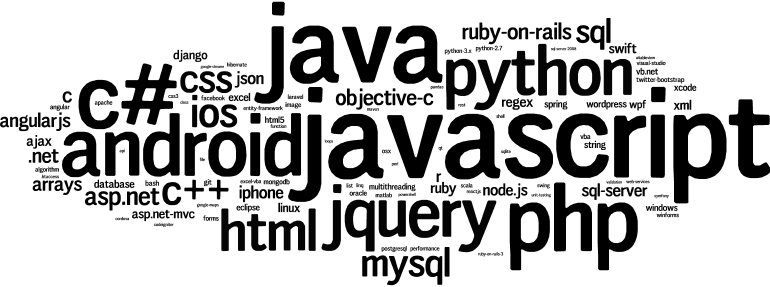
\includegraphics[width = 0.48\textwidth]{figures/toptagESO.png}
		\label{fig:ESOtag}}
	\hfill
	\subfigure[Russian Stack Overflow]{  
		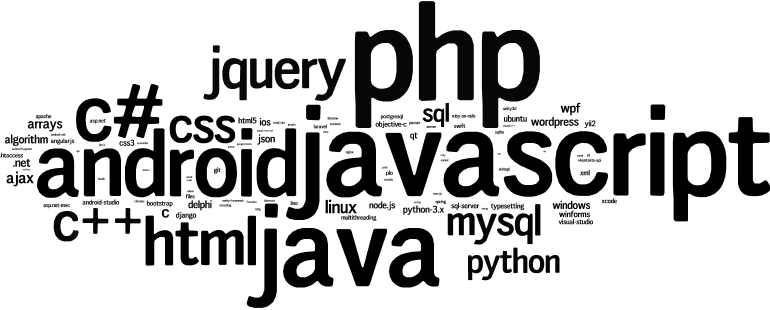
\includegraphics[width = 0.48\textwidth]{figures/toptagRSO.png}
		\label{fig:RSOtag}}
	\caption{Top-100 most frequently used tags in ESO and RSO}
	\label{fig:tagclouds}
\end{figure}

\begin{figure}
	\centering
	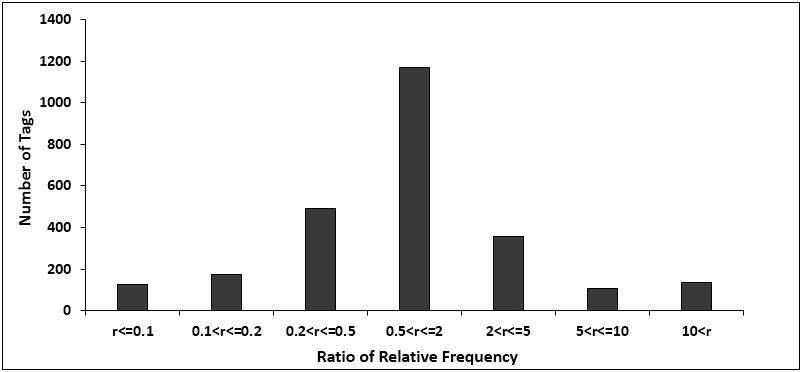
\includegraphics[width = 0.8\textwidth]{figures/relfreqbar.png}
	\caption{Comparative ratios ($r$) distribution of the common tags' relative frequency in RSO to its relative frequency in ESO}
	\centering
	\label{fig:relfreqbar}
\end{figure}

\begin{comment}
\begin{table}
	\small
	\centering
	\caption{Comparative ratios (r) of a common tag's relative frequency on Russian Stack Overflow to its relative frequency on English Stack Overflow \textcolor{blue}{1) use a bar chart. 2) feel that relative frequency ratio differ in 5 times is a too big difference. maybe 2 times is better? if so, split it into $r \leq 0.1$, $0.1 < r \leq 0.2$, $0.2 < r \leq 0.5$, $0.5 < r \leq 2$, $2 < r \leq 5$, $5 < r \leq 10$, $10<r$}}
	\label{tab:rel_freq}
	\begin{tabular}{llllll}
		\hline
		\textbf{r > 10} & \textbf{5 < r <= 10} & $\textbf{1 < r <= 5}$ & $\textbf{0.2 < r <= 1}$ & $\textbf{0.1 < r <= 0.2}$ & $\textbf{ r <= 0.1}$ \\
		\hline
		135 & 105 & 885 & 1135 & 173 & 127 \\
		\hline
	\end{tabular}
\end{table}
\end{comment}


%The tag is a means of connecting experts with questions, and they will be able to answer the question by sorting questions into specific and well-designed categories. 
%Research on the tags is able to reveal a number of most hot fields and topics in the Q\&A website content. 


%To check the overlap and difference of tags between Russian Stack Overflow and Stack Overflow, we first translate Russian tags into English with Google Translate, and then \textcolor{red}{manually revise some incorrect translations ??give some typical examples of such manual corrections?} to make them identical to the main site ones.
\subsection{Tag Uniqueness}
1397 of the 3957 tags in Russian Stack Overflow do not exist in English Stack Overflow.
That is, about 35.3\% technical terms are of interest by only RSO users such as \textbf{Yandx} (the largest Russian search engine in Russia like Google), \textbf{VKontakte} (biggest social network company in Russia like Facebook), \textbf{Denwer} (a popular local server in Russia), \textbf{bitrix} (a popular CMS in Russia written in php), etc.
As these techniques or services that these tags represent are Russian-specific, they are rarely used outside of Russia.
Therefore, ESO does not have questions about these techniques or services.
However, Russian Stack Overflow provides a perfect place to discuss such Russian-specific techniques or services.
These site-specific tags have been used to annotate 61,662 posts in RSO which account for 15.4\% of all 400,185 posts in RSO.

\vspace{2mm}
\noindent \fbox{\centering%
	\parbox{0.98\textwidth}{%		
		\textbf{Summary}:
		According to the tag usage analysis, the majority of tags in RSO are also in ESO.
		However, the level of usage frequency of the common tags often differs between the two sites, which reveals different level of interest in the corresponding technology.
		Furthermore, RSO also has its unique tags whose related posts make an non-negligible proportion of all posts in RSO.
		This shows that non-English speaking users do have unique knowledge needs and interests other than the knowledge in English.
	}%
}
\\

\begin{comment}
	%Ranking the top 10 frequent tags in several sets to show what are the most popular fields in both sites.
\begin{table}[!h]
	\scriptsize
	\centering
	\caption{Top 10 Popular Tags Ranking Statics \textcolor{red}{1) How is freq \% calculated? Need to explain in the discussion. 2) Tags only in Russian should be a separate table. They are not top-10 popular tags.}}
	\label{tab:table4}
	\begin{tabular}{|p{0.8cm}<{\centering}|p{0.55cm}<{\centering}|p{0.8cm}<{\centering}|p{0.55cm}<{\centering}|p{1.5cm}<{\centering}|p{0.55cm}<{\centering}|}
	\hline
	{\scriptsize Main site tags} & freq. (\%) &{\scriptsize Russian site tags} & freq. (\%) &{\scriptsize Tags only in Russian site} & freq. (\%) \\
	\hline
	javascript & 3.39 & php & 6.51  & bootstrap  & 0.304 \\
	\hline
	java & 3.04 & javascript& 5.83  &\bf vkontakte-api & 0.200 \\
	\hline
	c\# & 2.63 & java & 5.31 & android-sdk & 0.178 \\
	\hline
	php & 2.59 & android & 4.43 & android-fragment & 0.143 \\
	\hline    
	android & 2.38 & c\#& 3.89 & mvc & 0.139 \\
	\hline    
	jquery & 2.01 & html & 3.21 & google-maps-api &0.109 \\
	\hline    
	python & 1.87 & jquery& 2.82 & golang & 0.106 \\
	\hline    
	html & 1.59 & c++ & 2.75 & cookie & 0.105 \\
	\hline    
	c++ & 1.23 & css & 2.47  & cms & 0.102 \\
	\hline    
	ios & 1.22 & mysql & 2.08  & \bf yandex-maps-api & 0.092 \\
	\hline 
	\end{tabular}
\end{table}		
\end{comment}

\begin{comment}
\begin{table}[!h]
	\scriptsize
	\centering
	\caption{Different tags preference between two sites \textcolor{red}{why this set of tags as examples? Please tell how do you get this set of tags.} \textcolor{blue}{XINGZC: In addition to showing some examples, I think we need to perform some statistical analysis of the ranks of all 2560 common tags in the two sites, which can show that whether the level of interests in these techniques are statically the same or different.}}
	\label{tab:table_tagpref}
	\begin{tabular}{|l l l l l|}
		\hline
		{\scriptsize Tags} & freq. in SO (\%) & freq. in RSO (\%) & Rank in SO & Rank in RSO \\
		\hline
		web-application & 0.047 & 0.49 & 322  & 32 \\
		\hline
		yii2 & 0.03 & 0.45 & 518  & 35 \\
		\hline
		cuda & 0.029 & 0.012 & 528 & 870 \\
		\hline
		winforms & 0.2 & 0.5 & 63 & 29 \\
		\hline    
		Unity3D & 0.08 & 0.029 & 175 & 58 \\
		\hline    
		website & 0.02 & 0.485 & 734 & 31 \\
		\hline    
		layout & 0.057 & 0.42 & 287 & 41 \\
		\hline    
		Joomla & 0.037 & 0.125 & 424 & 145 \\
		\hline    
	\end{tabular}
\end{table}	
\end{comment}

%According to the result shown in Table~\ref{tab:table4}, it is clear that the most popular areas of two sites are very similar. Though there is some difference among the \textcolor{red}{frequency numbers of the same tag ??you mean absolute frequency number? they are not comparable as the two site are of very different scale, not just due to different preference?} due to the different preference of two sites' users. Overall, 8 of the top 10 most popular tags on Russian site are also the top 10 popular tags on the main site. This indicates that the popular area and content between two sites are highly overlapped. However, focusing on some unique tags in Russian site, it appears some tags who also own considerable frequency. For example, {\bf Yandx}, which is {\bf \foreignlanguage{russian}{Яндекс} }in Russian, is a Russian multinational technology company specializing in search engine and it is the most used search engine in Russia.{\bf []} And {\bf VKontakte}, another Russian local company, is the biggest social network company in Russia and its website, vk.com, is the most popular webstie in Russia.{\bf []} It shows that the Russian sub-site does have some specialness in the content area.
	\section{Community Split? Evidences of User Registration, Posting Behavior and Reputation Score}
%In this part, we mainly analyse whether it is necessary to build multilingual Stack Overflow by deeply compare the user activity, the knowledge base status and the areas of focus between Stack Overflow main site and Russian Stack Overflow site. The combination of all research results can lead to a solid conclusion for the meaning of multilingual Q\&A community development. \par 

\begin{comment}
For instance, Table~\ref{tab:multiSO} not only shows the number of posts, comments, users, but also the overlap users between each new site with the main site.
The high percentage of the overlap of users may negatively influence the main site, but is needs further quantitative analysis to be confirmed.

%\begin{table}[h!]
\begin{table}
	\centering
	\caption{Statistics of Stack Overflow main site and its lingual variants (By 8th Dec. 2017)}
	\label{tab:multiSO}
	\begin{tabular}{lrrrr}
		Site & \#User & \#Both Sites User & \#Post & \#Comment\\
		\hline
		Main site & 8,123,937 & * & 38,485,047 & 62,389,331\\
		Russian & 98,125 & 51,415(52.4\%) & 400,185 & 750,143\\
		Portuguese & 70,985 & 42,455(59.8\%) & 202,002& 361,108\\
		Spanish & 60,110 & 34,833(57.9\%) & 94,827 & 155,098\\
		Japanese & 14,777 & 7,818(52.9\%) & 30,571& 29,395\\
	\end{tabular}
\end{table}	
\end{comment}

Users, especially the core users are crucial to the success of Q\&A sites~\cite{mamykina2011design}, as they play an important role in asking and answering questions, and in curating post content and quality.
Will the multi-lingual sites result in the split of user community by the languages?
What kinds of users contribute the most to the multi-lingual sites?
Will multi-lingual sites affect the posting behavior of users who have accounts in both English and non-English sites?
We answer these questions by analyzing user registration, user reputation score, and user posting behavior.
%Some users have accounts in both Stack Overflow and Russian Stack Overflow.


\subsection{User Registration}
%\textcolor{red}{CCY: We tune-down the \textbf{migration} and avoid mentioning it in the paper.}
%Focusing on this intersection user base, the user migration can be measured by comparing their account creation dates of both site. 

By December 8th, 2017, there are 8,123,937 users in the English Stack Overflow (ESO) site and 98,125 users in the Russian Stack Overflow (RSO) site. 
As both sites belong to Stack Exchange networks~\cite{web:StackExchange}, we can identify the intersection of users who own both ESO and RSO accounts by their Stack Exchange ID.
We find that 51,415 users own both accounts at the same time, accounting for 52.4\% of the total number of the users in Russian Stack Overflow.

We further check the account registration time of these 51,415 users.
Among these 51,415 users, 32,288 (62.8\%) sign up their ESO account first and then sign up RSO account.
Those users account for 32.9\% of the 98,125 registered users in RSO which shows the importance of the ESO site to the development of the RSO site.
However, compared with the total 8.1 million users in ESO, 32,288 users account for only 0.4\%.
Therefore, even all of these 32,288 users stop using ESO and contribute only to RSO, it will not result in a significant loss for ESO.
Let alone many uses who own both accounts do not stop contributing to ESO after signing up RSO (see Section~\ref{sec:userpostingbehavior}). 
On the other hand, 19,125 (37.2\%) users sign up their RSO account first, and then sign up ESO account.
It means that to some extent, the launch of RSO may help to attract users to ESO.
This could further reduce the potential loss of users in the English site.

 
\begin{comment}
\begin{figure}[!h]
	\centering
	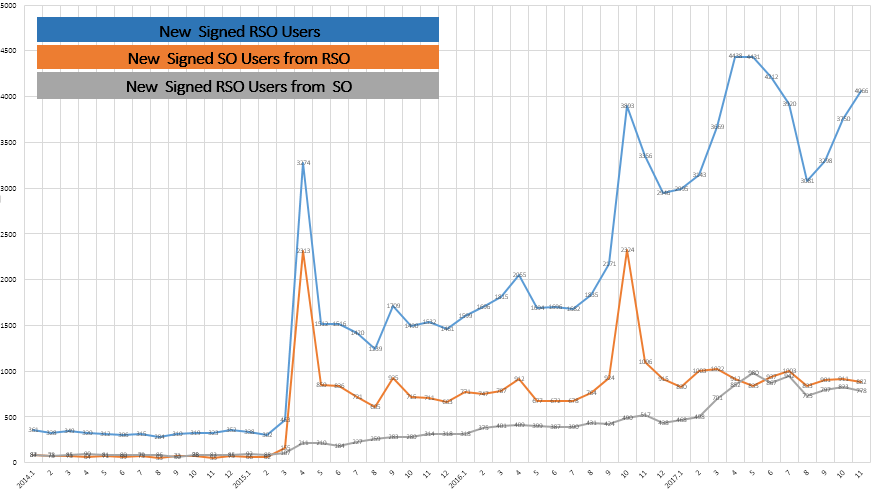
\includegraphics[width = 0.7\textwidth]{figures/userflow.png}
	\caption{The Sign Up for different sites}
	\centering
	\text{\scriptsize(SO for Stackoverflow and RSO for Russian Stackoverflow)}
	\label{fig:signup}
\end{figure} 
 
To illustrate the user migration in details, Figure~\ref{fig:signup} presents the statics of the users who sign up a Russian Stack Overflow account from Jan 1st, 2014 (the launch time of Russian Stack Overflow) to Dec. 8th, 2017. 
As shown in the figure, the new users who migrated from Stack Overflow main site 
occupy a high proportion, and also the Russian site attracts and \textcolor{red}{feedbacks a growing 
number of users ??what does this mean? not good English} to the main site with the time going by. 
In other words, the main 
site and the multilingual version both have a positive effect on the other one, which 
means both of them can \textcolor{red}{assist the development of the other ??this conclusion contradicts to that of last paragraph!}. This phenomenon means 
the development of multilingual version is helpful for the development of the main 
site.
%This phenomenon means the development of multilingual version is helpful for the development of the main site.	
\end{comment}

%\subsection {User Location}

Next, we would like to investigate the impact of building RSO site to the specific group of users in the original ESO site who can speak Russian.
To that end, we try to identify users in ESO who are from Russia or can speak Russian.
In Stack Overflow, users can create their own profiles by filling in their names, location, AboutMe (self introduction), GitHub link, etc.
Fig.~\ref{fig:userportfolio} shows an example user profile who can speak Russian.
We first check if the user's location is in Russia.
If the location contains any Russian letters, we regard the place as in the Russia.
If the location is written in English, we determine whether the location is in Russia by checking the Russian cities list on Encyclopaedia Britannica\footnote{\url{https://www.britannica.com/topic/list-of-cities-in-Russia-2040243}}.
We assume that the users whose location is in Russia can speak Russian.
%Through the location, we find \textcolor{red}{??} users who may be from Russia.
Then for other users who do not have location information, we further check if their AboutMe contains any Russian letters, and if so we also regard such users as ones who can speak Russian.

\begin{figure}
	\centering
	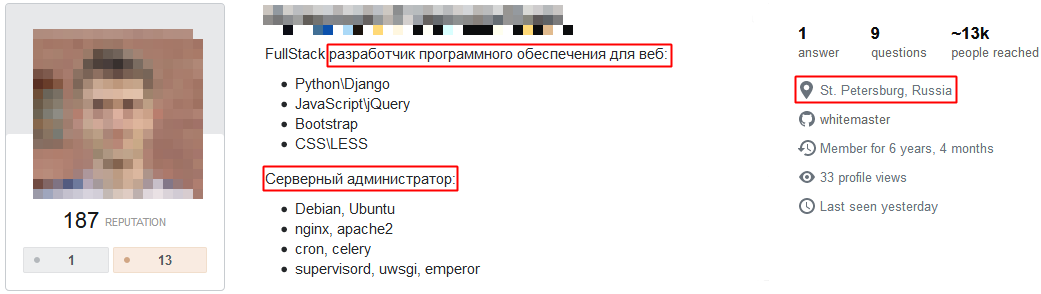
\includegraphics[width = 0.8\textwidth]{figures/userportfolio.png}
	\caption{One user portfolio in English Stack Overflow. This user may speak Russian.}
	\centering
	\label{fig:userportfolio}
\end{figure}

Using the above two heuristics, we find in total 34,705 users in ESO who may speak Russian.
Among these users, 10,699 (30.8\%) have registered RSO.
Within these 10,699 users, 6,537 (61.1\%) users sign up ESO first, and the rest 4,162 (38.9\%) users sign up RSO first.
While for the other users in ESO (8,089,232), only 40,716 (0.5\%) have RSO accounts.
The results show that, compared with users who do not speak Russian, RSO does attract many potentially Russian-speaking users in ESO. 
However, this does not mean a unidirectional loss of users from ESO to RSO, because RSO also helps attract users to ESO.
  
%It indicates that not only can Russian Stack Overflow attract users in Stack Overflow, but Stack Overflow can also benefit from Russian Stack Overflow.
%Such phenomenon mitigates the user loss of Stack Overflow.

\begin{comment}
To identity the Russian users on the Stack Overflow main site, the location information of registered users has also been analyzed. The users whose location are places in Russia (either written in English or in Russian) as well as the ones whose AboutMe sections contain Russians are marked as Russian related users, indicating their native language is probably Russian. The collected statistics is shown in Table~\ref{tab:loc}. Under this assumption, there are \textcolor{red}{34,705 Russian related users ??why not 51415 in Section 2.1.1?} registered on the Stack Overflow main site. Among these users, 10,699 (30.8\%) users have the Russian Stack Overflow account at the same time which means the rest majority of Russian users only use the main site. 
Also, within these 10,699 users, 6,537 (61.1\%) users migrated from main site to Russian site and 4,162 (38.9\%) users migrated from Russian site to main site. Most Russian related users (69.2\%) on the Stack Overflow still only have the main site account rather than migrating to the Russian Stack Overflow. 
 
\begin{table}[h!]
	\centering
	\caption{Location and AboutMe information analysis (users count among 8,123,937 main site users)}
	\label{tab:tablex}
	\begin{tabular}{lrr}
		Filter & \#Location Info. & \#AboutMe Info.\\
		\hline
		contain non-englsih word & 111,006  &  35,000\\
		contain Russian Letter & 9,858 &  2,079\\
		contain Russian Places & 24,468 & 1,718\\
	\end{tabular}
    \begin{tabular}{lr}
    	\hline
    	Total Russian related users: & 34,705\\
    	Russian related users with RSO account: & 10,699\\
    \end{tabular}
	\label{tab:loc}
\end{table}	
\end{comment}
 
\subsection{User Posting Behavior}
\label{sec:userpostingbehavior}

In a Q\&A website, the main user interaction is to ask and answer questions.
We regard both questions and answers as posts.
In RSO, there are 400,185 posts as of December 8th, 2017.
We count the number of posts created by different users.
The results can be seen in Table~\ref{tab:postnumber}.
We can see that 6,201 (6.3\%) users who have created more than 10 posts have contributed to 75.9\% posts in RSO.
So, we regard these 6,201 users as the core users in RSO.

\begin{table}
	\centering
	\small
	\caption{Statics of user posting behavior in Russian Stack Overflow}
	\label{tab:postnumber}
	\begin{tabular}{lllll}
		\hline
		\textbf{\#Post by User} & \textbf{\#Post} & \textbf{\% of All Posts} & \textbf{\#User} & \textbf{\% of All Users} \\
		\hline
		$>=$2 &372,046&92.9\%&24,908&25.4\%\\
		$>=$4 &345,543&86.3\%&13,526&13.8\%\\
		$>=$6 &328,398&82.1\%&9,644&9.8\%\\
		$>=$8 &314,833&78.7\%&7,537&7.7\%\\
		$>=$10&303,604&75.9\%&6,201&6.3\%\\
		\hline
	\end{tabular}
\end{table}	

\begin{comment}
Post is the prime part in the content of a Q\&A websites since post is the rising of the question as well as the origin of the answers and comment. It is also a very suitable variable to find the active users and popular topics in the Q\&A website community. Although every user has the right to post a question and add comments, the composition of the knowledge base ought to obey \textcolor{red}{the Pareto Law, which means 20\% of the users make 80\% of the contribution ??where do you find this? any reference or support? in general, literature says power law. how can know 20\% versus 80\%?}.

Imagine that a post is a single unit, and millions of posts consist of the knowledge base, and each post includes maybe a lot of answers and comments in the tree structure. 
From Table 1 it is already clear that there are totally 400,185 posts for the Russian Stack Overflow, and using the unique account id to calculate the amount of post for each user on Russian Stack Overflow, the results are presented in Table~\ref{tab:postnumber}. 	

From the table, the static distribution can be easily seen. As mentioned above, with the number of a single user post sum growing, the user proportion decrease. Notice that 6,201 (6.3\%) people from the 98,125 Russian Stack Overflow users who have 10 or more posts contribute 75.9\% of the post amount. These users could be labled as ´ Core User´ in this study representing the ones who have the highest level of contribution. Again, in these 6,201 core users, 1,845 people
are local users while 4,356 people own both main site account and Russian sub-site
account at the same time. In these 4,356 users in the intersection, 1,835 people are
migrants from the Stack Overflow main site. This distribution has been shown in Figure~\ref{fig:reputationTree}.

For the \textcolor{red}{1,676 ??where is this number from? never appear above?} of Core Users who sign up the Stack Overflow account first, which also known as the migrant from the main site, they post 104,448 posts on Russian sub-site that count 26.1\% of the post amount on Russian sub-site. For the \textcolor{red}{2,521 ??where is this number from?} of Core Users who sign up the Russian sub-site account first, which also known as the migrant from the main site, they post 139,275 posts on Russian sub-site that count 34.8\% of the post amount on Russian sub-site. According to the average level, the external users do not dominate the post area. 
\end{comment}

As shown in Fig.~\ref{fig:usercomponent}, 4,356 of the 6,201 core users own both ESO and RSO accounts. 
1,860 users sign up ESO first, but they created 139,275 posts in RSO which account for 34.8\% of all posts in RSO.
1,845 local users and 2,496 users who sign up RSO first created 260,910 posts in RSO which accounts for 65.2\% of all posts.
We can see that a large proportion of core users comes from ESO.
These core users make significant contributions to Russian Stack Overflow, but the local core users and the core users who sign up RSO first make even relatively more contributions. 
%It shows that although many core users may come from Stack Overflow they do not dominate Russian Stack Overflow.
%Actually most contributions come from local users in the Russian site.

\begin{figure}
	\centering
	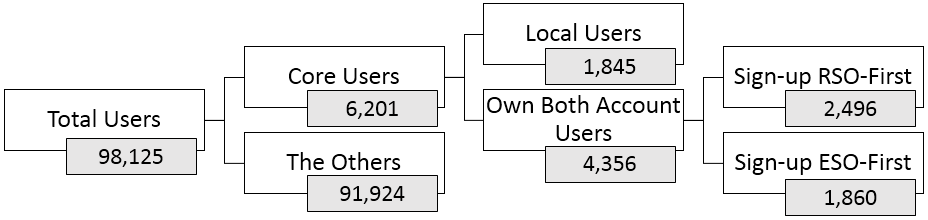
\includegraphics[width = 0.7\textwidth]{figures/usercomponent.png}
	\caption{User composition in Russian Stack Overflow}
	\centering
	\label{fig:usercomponent}
\end{figure}

If a core user in RSO who signs up ESO first and then RSO contributes comparatively less to ESO after signing up RSO, we say that RSO negatively influence this user's contribution to ESO.
To identify such users, we define the following formula: 

\begin{equation}
f = \frac{PostCountonESOAfterSignupRSO/DaysAfterSignupRSO}{PostCountonESOBeforeSignupRSO/DaysBeforeSignupRSO}	 
\label{equ:active}
\end{equation}

For a user who sign up ESO first and then RSO, this equation compares the user's average post number per day in ESO before and after the user signs up RSO.
The smaller value indicates that the user makes comparatively less contribution to ESO after signing up RSO.
%\textcolor{blue}{The smaller value represents the more possibility the user has migrated from Stack Overflow to Russian Stack Overflow. XINGZC: I think this formula alone tells only the posting behavior change on ESO after singing up RSO. Without contrasting it to the post behavior on RSO, i.e., average post per day on RSO, it cannot tell the migration from ESO to RSO. Maybe this users stop contributing to SO no matter ESO or RSO. Just like the stanislav example below, you need to study how many posts he contributes to RSO. Only if a user's contribution to RSO is comparable to his contribution to ESO before signing up RSO and his contribution to ESO decreases after signing up RSO, then we may guess this user migrate from ESO to RSO.}
%It means that if a core user in Russian Stack Overflow is more likely migrant if he creates fewer posts in Stack Overflow after his registration of the Russian one than that before his registration.
%\textcolor{red}{CCY to XINGZC:As all users analyzed here is core users, we assume they make big contributions to RSO. Once they contribute less in ESO after their RSO registration, we assume that they are migrating to ESO.}
Let's take one user as an example whose id is \textit{Vlad} in English Stack Overflow\footnote{\url{https://stackoverflow.com/users/276994}} and \textit{VladD} in the Russian one\footnote{\url{https://ru.stackoverflow.com/users/10105}}.  
He joined the ESO first on February 2010, and then joined the RSO on November 2012.
Before joining the RSO, he has answered 669 questions in ESO in about 2 years, but only answered 189 questions in ESO for 5 years after his join into RSO. 
Instead, he has answered 3,798 questions in RSO and earned 173,213 reputation score so far, while his current reputation score in ESO is only 28,781.
This user can be regarded as a user migrated from ESO to RSO.
%\textcolor{orange}{new example updated, whoes f value is around 0.37 but this user is a high reputation score users on both sites}

\begin{comment}
Moreover, for the 1,835 of Core Users who sign up the Stack Overflow account first,
according to their frequency of post activity, it can be also concluded that they are still
spending more time and concentrate on the Stack Overflow main site. The formula of
judging a migrant is Formula~\ref{equ:active}. If the f value is greater than 1, the user transferred his or her main active area to the new site.
\end{comment}


We consider $0.8 \leq f \leq 1.2$ as a reasonable range for relative stable level of contribution to ESO after the user signs up RSO.
That is, the user's posting behavior in ESO does not change significantly after signing up RSO if $0.8 \leq f \leq 1.2$.
%level that is 0.8 to 1.2 \textcolor{red}{1.2 ??why not 1?},since we consider that the user's active degree on English StackOverflow did not change significantly within this range.
%For $f$, the results in Table~\ref{tab:table3} reveal that more than half of those active users from the main site tend to be more active in a multilingual sub-site. Although they are from another site, they make a lot of contribution and seem to be like using the new sub-site regularly. 
%\textcolor{blue}{The following analysis needs to contrast $f$ with average post per day on RSO.}
%As seen in Table~\ref{tab:migrationCalculation}, 
Among 1860 core users in RSO who sign up ESO first, 120 (6.5\%) are with the $f$ value in range of 0.8 to 1.2, i.e., their contribution is relatively stable in ESO after signing up RSO.
1033 (55.5\%) users are even more active in ESO with $f>1.2$. 
Only 707 (38\%) users become less active in ESO.
It indicates that although many users from ESO contribute a lot to RSO, they do not stop making consistent contributions in ESO.
It further demonstrates that the launch of RSO will not cause severe community split of users between ESO and RSO. 
%The conclusion of the research on post aspect is the multilingual community has a group of users as backbone so that the community is not dominated by the users from the Stack Overflow main site, but the migrants from the main site are also willing to contribute in the new community.

\begin{comment}
\begin{table}
	\small
	\centering
	\caption{Posting Behavior Change for Core users Who Signs up ESO First then RSO \textcolor{blue}{I think we better not split the analysis by $>20, 50, 100$. For those $>50, 100$, most of f values decreases. This may means those most active users actually contribute relative less after signing up RSO. This is hard to explain.}}
	\label{tab:migrationCalculation}
	\begin{tabular}{lllll}
		\hline
		\textbf{\#RSO Post by User} & \textbf{\#User} & $\textbf{f < 0.8}$ & $\textbf{0.8<=f<=1.2}$ & $\textbf{f > 1.2}$ \\
		\hline
		$>=$10 & 1,860  &707 & 120 & 1033   \\
		$>=$20 & 445  & 208 & 39 & 198\\
		$>=$50 & 228 & 134 & 18 & 76 \\
		$>=$100& 134 & 94 & 11 & 29 \\
		\hline
	\end{tabular}
\end{table}		
\end{comment}

%\textbf{Summary:} The migrated users from Stack Overflow main site are not dominant in the Russian subsite.

\subsection{User Reputation Score}

%\textcolor{red}{
%I think we should have this reputation score analysis for those 6201 core users from the posting behavior analysis, rather than reputation score of users with an arbitrary reputation score cutoff 20. We should see how many local, users sign up ESO first, users sign up RSO first among these 6201 core users and then plot the R score of these 6201 core users in several intervals. 
%The current logic flow is awkward because we have two different ways to study users: active users with an arbitrary R score above 20, and core users who post more than 10. See also my comments below on the cutoff 20 and Fig.2.}
%\textcolor{blue}{CCY: 1) post number is not necessarily correlated to the reputation score as reputation score contains not only upvotes of posts, but also other post edits and tag wiki creation. So I want to see the power of ESO users in RSO from this aspect. 2)Yes, 20 is too arbitrary, have removed it.}
%\textcolor{red}{XINGZC: That is fine. But it may still be attacked.}
In Stack Overflow, users can earn reputation score if their questions, answers or comments get upvotes. 
They can also get bonus if they commit to editing others' posts, creating tag wiki which help to maintain the quality of the site.
So, apart from the number of posts, reputation score is another good indicator of how much contribution a user has made to the community and how much the community trusts his work.
%\textcolor{blue}{It has been used as a metric to identify active and credible users in the Q\&A sites~\cite{??findsomereferences,??,??} XINGZC: This may invite questions that why we do not use reputation score to identify users for posting behavior analysis?}.
%Figure~\ref{fig:reputationDistribution} shows the distribution of reputation score of 98,125 users in Russian Stack Overflow.
According to the privilege policy of Stack Overflow\footnote{\url{https://stackoverflow.com/help/privileges}}, users who earn more than 10 reputation score can remove the new user restriction. 
%To focus on the reputation distribution among the formal users, this section only includes 31,029 users with more than 10 reputation score on Russian Stack Overflow.}
As new users do not contribute much to the site, we only consider 31,029 users with more than 10 reputation score in RSO in this analysis.
These 31,029 users in RSO belong to three groups:
10,702 (34.5\%) local users who only register RSO,
12,292 (39.6\%) users who sign up ESO first and then sign up RSO,
and 8,035 (25.9\%) users who sign up RSO first and then sign up ESO.

\begin{figure}
	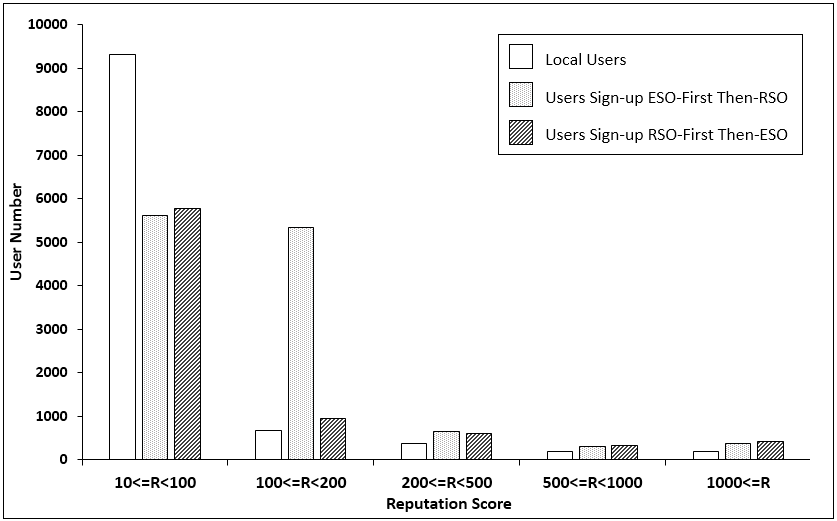
\includegraphics[width = 0.6\textwidth]{figures/reputation.png}
	\caption{The reputation distribution of three-group users in RSO}
	\label{fig:reputationDistribution}
\end{figure} 

Fig.~\ref{fig:reputationDistribution} shows the distribution of reputation score of these three groups of users in five different intervals.
We can see that the distributions of reputation score in the first two low-reputation intervals are different from those in the three high-reputation intervals.
This phenomenon is due to the Association Bonus Policy of Stack Exchange~\cite{web:associationBonus}.
According to this policy, a user will earn 100 bonus reputation score in RSO when the user signs up a RSO account, if the user has already owns an ESO account with 200+ reputation score.
Therefore, compared with local users and bi-account users who sign up RSO first, there is a relatively less proportion of bi-account users who sign up ESO first in the reputation interval $10 \leq R < 100$.
In contrast, a large proportion of bi-account users who sign up ESO first have reputation score within $100 \leq R \leq 200$.
This results in that the number of bi-account users who sign up ESO first is more than the sum of local users and bi-account users who sign up RSO first in the interval $100 \leq R \leq 200$.

But in the other three intervals (i.e., $R \geq 200$), we can see that the number of local users plus the number of users who sign up RSO first then ESO is more than the number of users who sign up ESO first.
%the number of users sign-up ESO-first then-RSO is roughly the same as the number of users sign-up RSO-first then-ESO
Furthermore, in the three intervals $R \geq 200$, there are roughly the same number of users in the group of users sign up ESO first and in the group of users sign up RSO first.
However, considering that there are 12,292 users in total who sign up ESO first and 8,035 users who sign up RSO first, the later group has much higher percentage of high-reputation users than the former group.

This analysis suggests that the community of RSO has its own core contributors.
However, its community is not completely independent of that of ESO, because a large number of users from ESO (especially high-reputation users from ESO) makes similar contribution to RSO, as those local users and those who sign up RSO first.	

\begin{comment}
Considering the Reputation Bonus Policy that a starting plus 100 reputation bonus 
to users who already have a 200+ account of any site belongs to Stack Exchange [5], the 32,288  users who migrated from the main site reasonably have a large number of 
the reputation level of 100 to 200. However, despite the local user, the remains are 
the user who owns both account of the main site and Russian version. Under the 
circumstance that the number of migrants is almost \textcolor{red}{2 times ??32288/19125 about 1.7 times, not 2. In a technical paper, has to be very specific} of that of the 19,125 users 
who sign up Russian version account first, \textcolor{red}{the later contributes somehow an equal 
number of active users ??how can we tell this from Fig. 3?}.

To some degree, the reputation reveals that multilingual communities \textcolor{red}{are not dominated 
by a large number of external users even the later has an overwhelming advantage 
on the user amount ??do not understand how this conclusion can be reached from the reputation distribution analysis?}, which means that multilingual communities are relatively 
independent in the respect of user contribution in the community development process.
\end{comment}


%In Stack Exchange, once a user get more than 200 reputation points, he will get site %association bonus i.e., 100 points on each site in Stack Exchange, as Stack Exchange regards %that user as trusted [5]
%~\cite{https://stackoverflow.com/help/whats-reputation}.
%Therefore, we regard users with 200+ reputation score in Russian Stack Overflow as its core %users.
%Considering the Reputation Bonus Policy that a starting plus 100 reputation bonus to users who already have a 200+ account of any site belongs to Stack Exchange [5], the 29,609 users who migrated from the main site reasonably have a large number of the reputation level of 100 to 200. 

%However, there are 384,304 core users in Stack Overflow, and only 885 of them migrate to %Russian Stack Overflow.
%Figure~\ref{fig:reputationDistribution} displays the detailed reputation score distribution, %and most migrated user actually lay in the range between 100 to 200.
%That is because the core user in Stack Overflow can get 100 reputation points once they join %Russian Stack Overflow, but they are not counted as active in the new site as they are not %active to get another 100 points.  
%Among 3,390 core users, only 885 (28.24\%) of them come from Stack Overflow.
%It demonstrates again that Stack Overflow is merely hurt by the launch of Russian Stack %Overflow, and Russian Stack Overflow is rather independent.
%However, despite the local user, the remains are the user who owns both account of the main site and Russian version. 


%\textcolor{red}{Actually, it is wrong to define migration as in this paper, because although some people come from Stack Overflow, they can only be regarded as migrated only if they are active in Russian Stack Overflow, but not active in the main site any more. But we do not have enough time to revise it.}

%\textbf{Summary:} 28.24\% core users in Russian Stack Overflow migrate from Stack Overflow.
%Under the circumstance that the number of migrants is almost 2 times of that of the 16,155 users who sign up Russian version account first, the later contributes somehow an equal number of active users.
%To some degree, the reputation reveals that multilingual communities are not dominated by a large number of external users even the later has an overwhelming advantage on the user amount, which means that multilingual communities are relatively independent in the respect of user contribution in the community development process.

\begin{comment}
Those are also people being targeted by the new site. So far for the argument that every decent programmer has to know English, some know it but just prefer their native language and I'd argue Matz is a more than decent programmer. As for most information being available in English and non-English information being bad, the first **public** release of ruby was in 1995 and by 2000 it was more popular than Python in Japan. The first English mailing list was created in 1999 but it took until 2002 for it to get as much messages as it's Japanese counter part (even though people from everywhere around the world could use it instead of just Japanese people). It actually took until Ruby 1.8 and 2003/2004 to get good documentation and books in English. That said we now got decent information about it in English available but there's also a massive Japanese community with wealth of information still, as one example Matz's own blog.	
\end{comment}

\vspace{2mm}
\noindent \fbox{\centering%
	\parbox{0.98\textwidth}{%
	   \textbf{Summary}: In term of post contribution and reputation score, Russian Stack Overflow benefits a lot from English Stack Overflow as many users in RSO come from ESO, especially those who can speak Russian.	
	   But there is no significant community split between the two sites, as those from-ESO users only account for a very small proportion of the user base in ESO and the majority of them still make stable contributions to ESO even after they sign up RSO.
	   In addition, RSO also helps to attract new users to ESO.    
	}%
}
\\

	\section{Knowledge Fragmentation and Duplication? Evidences of Cross-Site Linking}
%\textcolor{blue}{XINGZC: revised introductory paragraph and section 6.2.1. please check.}

ESO and RSO are both programming-related website and our tag usage analysis shows that users of the two sites share much common interests.
Therefore, it is reasonable that some new questions asked in the Russian Stack Overflow may have been already answered or have highly related questions in English Stack Overflow.
This could create knowledge fragmentation and duplication across multi-lingual sites.
But the supporters of multi-lingual sites argue that it is likely that users on non-English Stack Overflow may cross-reference posts to English Stack Overflow, which would solve the knowledge fragmentation and duplication issue.
Below is a user's comment about the concern of knowledge fragmentation and duplication and the suggestion that cross-site linking could solve the issue.	
\begin{comment}
In Q\&A discussions, users often cross-refer existing posts using hyperlinks~\cite{??dehengemseknowledgenetwork}, for example, linking to duplicate questions or related knowledge.
As our tag analysis shows that users of the two sites share some common interests, it is reasonable to expect that some questions in Russian Stack Overflow may have duplicate or related questions in English Stack Overflow.
This could create knowledge fragmentation and duplication across multi-lingual sites.
But the supporters of multi-lingual sites argue that it is likely that users on non-English Stack Overflow may cross-reference posts on English Stack Overflow, which would solve the knowledge fragmentation and duplication issue.
Below is a user's comment about the concern of knowledge fragmentation and duplication and the suggestion that cross-site linking could solve the issue.	
\end{comment}


\begin{comment}
Hyperlink is a good tool to recommend and refer the existing content to other users. 
%Not only links can refer the knowledge base in the same site, but also across different sub-sites, or external resources. 
%Under the site announcement of Japanese Stack Overflow, one user commented, ``''
As Stack Overflow and Russian Stack Overflow are both programming-related website, it is expected that some new questions asked in the Russian Stack Overflow may have already answered or highly related to Stack Overflow.
So there should be some mutual links between them.
In this section, we try to validate such assumptions with the analysis of existing links between them.
%In this section, we explore the relationships between Stack Overflow and Russian Stack Overflow according to their mutual hyperlinks. 
%The link amount and the direction reveal the similarity and difference between these two sites.
\end{comment}

\vspace{2mm}
\noindent \fbox{\centering%
    \parbox{0.98\textwidth}{%
        \textit{``This is the world wide web and it is built on a thing called hypertext. Multiple languages? Cool, that's the "world" part. But don't forget about hypertext. Please, make sure that questions and answers can be linked easily across the different language sites. If someone asks a question in Japanese that is essentially a duplicate of an existing English question, linking the two questions will allow Japanese speakers (who might understand *some* English, or at least be able to read code snippets) to get immediate value from past answers, without waiting for new answers... ''
        }
        
        {\raggedleft --- one comment on the announcement of Japanese Stack Overflow~\cite{web:SOjapanese}\par}
            }%
}
\\

In this section, we investigate existing cross-site links made by the users on Russian Stack Overflow and potential cross-site links that the users are not aware of.
This will provide evidences whether knowledge fragmentation and duplication is a serious issue for multi-lingual sites, whether manual cross-site linking is sufficient to battle this issue, and what kind of tools could better support cross-site linking.

\begin{table}
	\caption{Links statics}
	\centering
	\small
	\label{tab:links}
	\begin{tabular}{llll}
       \hline
		\textbf{Source}      & \textbf{\#Total links} & \textbf{\#Links to ESO}   & \textbf{\#Links to RSO} \\ 
		\hline
		ESO Posts     & 13,636,973    & 1,581,888 (11.6\%)      & 88 \\
		ESO Comments  & 5,959,110     & 1,835,405 (30.8\%)    & 164\\
		RSO Posts    & 131,964       & 5,674  (4.3\%)        & 5,014 (3.8\%) \\
		RSO Comments & 55,471        & 4,548  (8.2\%)        & 5,658 (10.2\%) \\
       \hline
	\end{tabular}

\end{table}	



\subsection{Explicit Cross-Site Links by Users}
\label{sec:explicitLink}
%\textcolor{blue}{ZCXING: not yet revise this section as it is not ready yet.}
%\textcolor{red}{CCY to ZCXING, I know that you are familiar with links in Stack Overflow. Is it suitable for us to categorise links as ``identical'', ``related'', ``un-related''? In addition, someone is saying I tries one link before, but it cannot solve my problem, what kind of link can we count it? Could you please have a look at the part below.}
%\textcolor{blue}{XINGZC: can be four categories: duplicate, related-helpful, related-but-not-helpful, unrelated.}

In Stack Overflow, users can add hyperlinks in their posts (both questions and answers) and comments to reference to other resources. 
We collect all hyperlinks in ESO and RSO and analyse the link direction within and across the two sites.
The statistics of hyperlinks in the two sites are summarised in Table~\ref{tab:links}.
We can see that a large proportion of hyperlinks in ESO posts and comments references to its own content, while only a few hyperlinks in ESO posts and comments reference to the RSO content.
This is unsurprising because English speaking users would not have much interest in Russian content.
In contrast, comparable proportion of hyperlinks in RSO reference to its own content and the ESO content, respectively.
This phenomenon indicates that there could be certain level of knowledge fragmentation and duplication between the two sites and RSO users attempt to address the issue by cross-site linking.

\begin{comment}
The hyperlinks in ESO rarely reference to RSO.
In contrast, many hyperlinks in RSO reference to ESO.
For example, in RSO, 4.3\% hyperlinks in posts and 8.2\% hyperlinks in comments reference to some posts in ESO.
However, compared with RSO, we can see that 11.6\% links in posts and 30.8\% links in comments are from itself in ESO.
%\textcolor{red}{CCY: this argument is a little far-fectched, how to say that more naturally in the paper?}
Such a large difference of link sources leads to two potential reasons: 1) There is not enough overlap content between two sites; 2) ESO may be under-referenced in RSO.
\end{comment}

%In RSO, one question may contain a link to posts (question or answer) in ESO.
%Our task is to see if that assumption holds by checking the retrieval result of our searching model mentioned above.
To further confirm this phenomenon, we manually examine the relationships between a RSO post and an ESO post that is referenced by a hyperlink in the RSO post.
We collect in total 5674 hyperlinks in RSO that reference to ESO.
For each hyperlink, we collect its residing RSO post and the ESO post being referenced.
As we are most familiar with \textit{Python} related questions, we randomly select 50 such pairs of RSO-ESO posts tagged with \textit{Python}.
Examining these 50 pairs of RSO-ESO posts reveal three kinds of relationships between a RSO post and its hyperlinked ESO post: 
duplicate questions (14 pairs), 
related and useful for problem solving (30 pairs), 
and related but not useful for problem solving (6 pairs).

%We assume that such a link represents that the source question in RSO has certain relationship with the target question in ESO.
%According to our observation, there are two kinds of different relationships among these links.
%\textcolor{red}{CCY: Please give detailed number for each category.}

%To systematically define the relationship between each link pair, we categorize the 50 links into three different categories, i.e., identical questions, similar question and not directly relevant questions. 
First, hyperlinks in 14 (28\%) RSO posts reference to some duplicate questions in ESO.
%The identical questions correspond to the refered English Stackoverflow questions which ask the basically same thing as the Russian one. 
For example, the Russian question \foreignlanguage{russian}{"как запустить скрипт на pypy?"}(postid=722948, ``how to run a script on pypy'') has a hyperlink to the English question ``How to use PyPy on Windows?'' (postid=9893317).
Both the Russian question and the English question are about how to run a script of pypy on Windows. 

Second, hyperlinks in 30 (60\%) RSO posts reference to some related but not duplicate English posts in ESO that are useful for solving the problem in the Russian questions.
%In term of the similar question, the pair of the two question ask about the highly relative question under a same topic. 
For example, the Russian question \foreignlanguage{russian}{"Обновление Label из цикла в tkinter"}(postid=581331, ``updating the label of the cycle in tkinter'') has a hyperlink to an ESO post ``Update Tkinter Label from variable'' (postid=2603169). 
The Russian question asks how to use the \textit{update}  function on Tkinter Label in a loop structure.
The referenced ESO question does not solve this specific problem, but it discusses how to use the \textit{update} function, which is relevant. 
%Although they are not duplicate question, they are related and the creator can use that link to help describe their question.
%Tough, the Russian question owner still refered this similar English question to help describe his own question. 
%So we consider this kind of refered questions under a same topic as similar questions.
%But we also find that some reference link are not right or relevant, which are marked as not directly relevant questions.

Third, sometimes RSO users add hyperlinks to the ESO posts in their questions to tell that they have examined some related ESO posts, but these ESO posts cannot solve their problems.
This kind of RSO posts accounts for 6 (12\%) of the 50 examined samples.
%\textcolor{orange}{The original result is just the model output (if model cannot find link pair in top10 result then consider it is related but not helpful), I redo the classification and involved manually checking this time. Data Updated.}
Fo example, one Russian question with the title \foreignlanguage{russian}{"Почему не работает унаследованная форма?"} (postid=318618 `Why does not the inherited form work?'') has a hyperlink to an ESO question ``why does not work in the form of validation?'' (postid=23534615).
The Russian question states that the answers to this ESO question do not work for his problem. 
%After checking these two question, we find that the Russian question wants to find a solution to solve his problem but he mentioned that the method in the referred English question was not working. 

To sum up, the first category of cross-site links reveals knowledge duplication, and the second category may have the risk of knowledge fragmentation.
However, the third category has nothing to do with knowledge fragmentation and duplication.


\begin{comment}
For instance, there is a Russian question, \foreignlanguage{russian}{"Почему нет исключения TypeError?"} (\#564442 "Why is there no TypeError exception?").
Its link in this question leads to the ESO question with title "In Python, how do I determine if an object is iterable?" (\#1952464). 
After manually checking this one pair on the Stack Overflow, we find that he question's owner mentioned one possibility causing the error and \textcolor{red}{refered the link to explain his assumption ???CCY: Do that mean they are related?}. 
So this refered English question is talking about another topic which actually can not deal with this error. So this reference link is not the most suitable one to descripe or solve this russian question.
\end{comment}


%Third, \textcolor{red}{??} links are not right or not suitable in the posts.
%\textcolor{red}{CCY: Give an example about it. }

\begin{comment}
Second, the reference which can not be spotted by our method is due to the limitation of our model. 
Our model focus on capturing and computing the semantic difference between the input words, so currently it may not work well with some deep semantic relationship between words. 
For instance, given an RSO question "\foreignlanguage{russian}{Порядок удаления элементов списка в python}"\footnote{\url{https://ru.stackoverflow.com/questions/55464/}} (translated as "the removal of elements of the list in python"), 
the link inside leads to an English question, "Calling 'del' on a list"\footnote{\url{https://stackoverflow.com/questions/8205102/}}.
In this example, 'del' is obviously a function name for deleting.
However, currently, our model is not able to capture such domain-specific information.
\end{comment}


\subsection{Implicit Cross-site Links that Users Are Not Aware of}
\label{sec:implicitLink}
In Table~\ref{tab:links}, we find that the ratio of hyperlinks in RSO posts and comments that reference to RSO and ESO posts is relatively lower than that of hyperlinks in ESO post and comments that reference to ESO and RSO posts.
This makes us hypothesize that there could be cross-site links between RSO and ESO posts that users are not aware of, and thus have not been explicitly hyperlinked.
%Apart from the existing links mentioned in last subsection, many posts in RSO may also need to add links to ESO, but not done due to the language gap.
To test this hypothesis, we carry out another empirical study. 
As ESO has millions of questions and answers, it is impossible to manually find if a RSO question has some related posts in ESO.
Therefore, we develop a cross-site retrieval method to locate potentially related questions in ESO, given a RSO question.
Then, we analyze the relationships between the given RSO question and the retrieved ESO questions to understand implicit cross-site links.
%Last section analyzes the existing links between two sites, and we are now investigating that if a post 

%But as both Stack Overflow and the Russian one own millions of questions and answers, it is difficult for us to observe to determine which reason accounts for the relative small proportion of links to Stack Overflow.
%Therefore, we propose a cross-site retrieval method to assist our observation and validate the reason mentioned above.

%To understand the scale of implicit cross-site links that the RSO users are not aware of, we develop a cross-site question retrieval method, inspired by~\cite{??bowencrosslingualretrievalemse2017}, to retrieve potentially related questions on English Stack Overflow given a Russian Stack Overflow question.

\begin{figure}
	\centering
	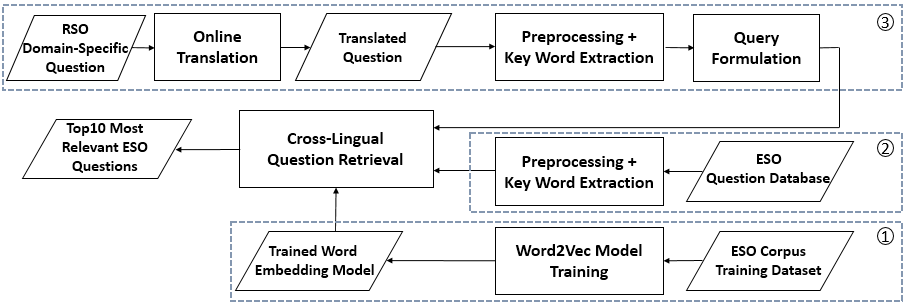
\includegraphics[width = 0.9\textwidth]{figures/workflow.png}
	\caption{Overall framework for cross-site retrieval}
	\centering
	\label{fig:flowChart}
\end{figure}

\begin{figure}
	\centering
	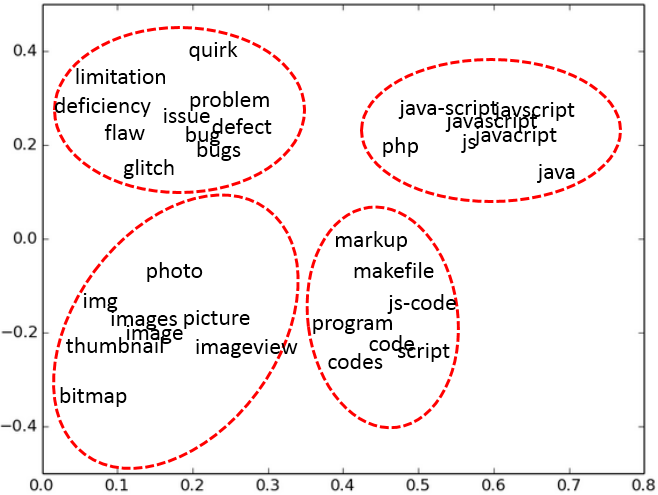
\includegraphics[width = 0.6\textwidth]{figures/PCAplot.png}
	\caption{Visualization of word embeddings by principle component analysis~\cite{jolliffe1986principal}}
	\centering
	\label{fig:PCAimg}
\end{figure}

\subsubsection{Method for cross-site question retrieval}
Fig.~\ref{fig:flowChart} displays the flow chart of our cross-site retrieval method.
The method can be divided into three main parts.
In the first part, we pre-train a word embedding model for retrieving related question for a given query. 
Word embedding~\cite{mikolov2013distributed} is a method to convert the words into dense vectors based on the assumption that words appear in similar context tend to have similar meanings. 
We train a word embedding model using all posts collected from ESO including both question titles and descriptions.
We adopt the Principle Component Analysis~\cite{jolliffe1986principal} to reduce the high-dimensional word embedding into 2-dimension for manual observation.
Examples of some word embeddings are visualized in Fig.~\ref{fig:PCAimg}.
We can see that similar words are close to each other in the vector space, such as ``js'' and ``javascript'', ``image'' and ``picture'', ``bug'' and ``defect''.
In addition, word embedding model is also robust to word morphological transformation (like plural ``images'', ``bugs'') and misspellings (e.g., ``javacript'' and ``jascript'' for ``javascript'').  
Compared with traditional keyword matching, word embedding model helps to bridge the lexical gap between different words which share similar meanings~\cite{chen2016learning}. 

In the second part, we prepare the posts from English Stack Overflow as a question database.
In this study, we build a database of 779,370 ESO questions tagged with \textit{Python}.
We pre-process each question by tokenzing the sentence and removing the stop words in both question title and description.
All words in the question title are considered as keywords.
We extract keywords from the question description because the question description contains too many technical details that could negatively influence the retrieval accuracy. 
We use two different popular keywords extraction algorithms (TF-IDF and TextRank) to extract keywords from the question description. 
TF-IDF (term frequency-inverse document frequency)~\cite{sparck1972statistical} is a numerical metric corresponding to the importance of a word in a corpus.
The TF-IDF metric of a word is proportional to the frequency of the word appearing in one post and inverse proportional to the number of posts in which the word appears.
TextRank~\cite{mihalcea2004textrank} is a popular unsupervised approach for automatic keywords extraction. 
It performs random walk on a graph of word co-occurrences to determine the most important words in a post.
These two algorithms yield two different but complementary sets of keywords. 
To reduce the bias of using a single algorithm, we choose the union of the two keyword sets to build our final set of keywords.
If a keyword appears in both title and description, we consider it as a title keyword.

In the third part, we formulate a RSO question as a query to retrieve related ESO questions in the ESO question database.
We first translate the RSO question's title and description into English with Google Translate~\cite{web:googleTranslate}.
We use the same pre-processing and keyword extraction steps to build a query from the given RSO question.
%We assign different weights to the query keywords from  title and description. 
As question title represents more compact and meaningful information than question description, we assign double weight to title keywords in the query than description keywords.
Given the query of a Russian question ($R$) and an English question ($E$) in the ESO question database, We define the relevance between a query keyword ($R_i$) and a question keyword ($E_j$) as the cosine similarity between the word embeddings of $R_i$ and $E_j$, i.e., $Rel(R_i, E_j)=CosineSim(v_{R_i}, E_j)$. 
For each query keyword $R_i$, we compute its relevance with each keyword of the English Question and find the one with the largest similarity: 
\begin{equation}
Rel(R_i,E)=\max\limits_{j \in E}Rel(R_i, E_j)\times R_i.Weight
\end{equation}
Note that this relevance is weighted by the query keyword's weight $R_i.Weight$.
We then define the relevance between the query of a Russian question ($R$) and an English question ($E$) in the ESO question database as:
\begin{equation}
\label{equ:relevance}
Rel(R, E) = \sum_{i \in R}Rel(R_i, E)
\end{equation}

We compute the relevance of the query and all questions in the ESO question database, and return the top 10 questions with the highest relevance as the most relevant English questions to the given Russian question.

\begin{comment}
%Each question contains two parts, title and descriptions.
\begin{enumerate}
 \item Given one question in Russian Stack overflow, we first translate its title and content description into English with Google Translate\footnote{\url{https://cloud.google.com/translate}}.
 Then we pre-process the translated question by tokenzing the sentence, removing the stop words in both question's title and description.

 \item \textcolor{red}{This step description is wrong! It mixes the two steps in Bowen's approach: 1) build a domain-specific term vocabulary; 2) extract keywords from the question description. I think this need to be separated, otherwise it reads very strange.}
 We extract keywords from the question description because the question description contains too many technical details that could negatively influence the retrieval accuracy. 
 We use two different popular keywords extraction algorithms (TF-IDF and TextRank\footnote{\url{https://github.com/davidadamojr/TextRank}}) to extract keywords from the \textcolor{blue}{ESO question corpus ??should be question description?}. 
 These two algorithms yield two different but complementary sets of keywords. 
 To reduce the bias of using a single algorithm, we choose the union of the two keyword sets to build our final keywords extraction vocabulary.
 Then we only select the keywords which appear in the vocabulary among the query description to improve the retrieval accuracy and speed.
 
 \item We assign different weight to the keywords in title and description. As title represents more compact and meaningful information, we assign double weight to title keywords than description keywords.
 
 \item To build the retrieval model, we adopt the word embedding model. Word embedding~\cite{??} is method to convert the words into dense vectors based on the assumption that words appear in similar context tend to have similar meanings. We trained an word embedding model on posts of Stack Overflow, and some examples can be seen in Fig.~\ref{fig:wordEmbedding}. \textcolor{red}{Add a picture about word2vec + PCA} We can see that similar words \textcolor{red}{....} are relatively close in the vector space. Compared with traditional keyword match, word embedding model can help bridge the lexical gap between different words which share similar meanings. To calculate the relevance between the Russian query ($R$) and an English question ($E$) from the database, we first define the semantic similarity between a query word ($R_i$) and a question word ($E_j$) as the cosine similarity between their learned word embeddings, i.e., $Rel(R_i, E_j)=CosineSim(v_{R_i}, E_j)$. For each query word $R_i$, we compute its similarity with each word in the English Question and find the one with the largest similarity: 
 	 \begin{equation}
       Rel(R_i,E)=\max\limits_{j \in E}Rel(R_i, E_j)\times R_i.Weight
     \end{equation}

     We then define the relevance between a given query \emph{R} and an English question from database \emph{E} as 
      \begin{equation}
      	 \label{equ:relevance}
         Rel(R, E) = \sum_{j\in R}Rel(R_j, E)
      \end{equation}
     We will compare the query with all questions in our database, and sort the relevance value calculated by Equ.\ref{equ:relevance}.
     10 questions with the highest value are extracted as the most relevant questions.
 \end{enumerate}
\end{comment}


\subsubsection{Manual validation of cross-site reference}
%\textcolor{blue}{ZCXING: not yet revise this section as it does not seem ready.}
%There are totally 779,370 questions tagged with \textit{Python} from ESO as the candidate for the query.
%Then we take the question (title and description) in Russian Stack Overflow as the query, and our model returns top-10 related questions in Stack Overflow.
%First, we use the 50 RSO questions in Section~\ref{sec:explicitLink} as query questions and obtain the top-10 related ESO question using our cross-site retrieval method.
We randomly sampled 50 RSO questions tagged with \textit{Python} that do not have hyperlinks to ESO. 
We use these RSO questions as query questions and obtain the top-10 related ESO questions for each RSO question using our cross-site retrieval method.
We then examine if the retrieved ESO questions are duplicate or otherwise related to the query RSO questions.  
%We regard them as the queries, and to see if we can find any identical or related questions in Stack Overflow in the top-10 retrieval results.
 
We find that for 6 (12\%) RSO questions, we can locate duplicate questions in the top-10 ESO questions returned by our cross-site retrieval method. 
For the other 20 (40\%) Russian questions, we can locate at least one related-but-not-duplicate ESO questions in the top-10 list. 
Table~\ref{tab:reviewresult} presents three RSO questions (title translated into English) in our study.
We only show the top 3 most relevant ESO questions due to the space limit. 
Among these three examples, our cross-site retrieval method finds a duplicate ESO question (postid=9694065,  ``Searching for a Python lightweight IDE (or text-editor)'') to the RSO question (postid=464, ``IDE for Python'') and finds some related ESO questions to the RSO questions (postid=432934, ``The slow implementation of the code a coin toss, and postid=420125, ``Books and educational resources for Python'').

For the rest 24 (48\%) RSO questions, Our cross-site retrieval method does not find any related questions in the current ESO database.
Note that it may be either due to the limitation of our method, or the fact that there are no duplicate or related questions in ESO. 
More future works are needed to confirm the detailed reasons.

 \begin{table}
 \caption{Examples from implicit cross-site links that users are not aware of}
 \centering
 \tiny
 \label{tab:reviewresult}
 \begin{tabular}{|p{0.8cm}|p{3.9cm}|p{3.9cm}|p{3.9cm}|}
 	%\hline
	%Russian Question &{\emph \foreignlanguage{russian}{IDE для Python}} & {\emph \foreignlanguage{russian}Отладка кода на Питоне}} &{\emph \foreignlanguage{russian} {Python обработчик системного меню Windows}\\ 
 	\hline
 	Translated Question & IDE for python (\#464) & the slow implement of the code, a coin toss (\#432934) & books and educational resources for python (\#420125)\\
 	\hline
 	Result \#1 & [duplicated] Searching for a Python lightweight IDE (or text-editor) (\#6011678) &  [related] python code for coin toss issues (\#6486877) & [related] Resource/book suggestion to effectively writing software for python/c++ beginner (\#9694065)\\
 	\hline
 	Result \#2 & [related] What's a good IDE for Python on Mac OS X? (\#893162) & [related] python coin toss (\#14882530) & [related] good resource for learning advanced or obscure python concepts (\#14756145) \\
 	\hline
 	Result \#3 & [related] IDE for Python: test a script (\#6023377) & [related] Simulate multipe coin toss streak (\#15761259) & [related] what are good online resources to learn using Pyhton to get and post data in a webpage? (\#41241481)\\
	
 	\hline
 \end{tabular}
 
 \end{table}

\vspace{2mm}
\noindent \fbox{\centering%
	\parbox{0.98\textwidth}{%

      \textbf{Summary}: 
      There are certain level of knowledge fragmentation and duplication across ESO and RSO.
      RSO users recognize some duplicate and related ESO posts and reference them in RSO posts and comments.
      But there are many duplicate and related ESO questions that RSO users are not aware of and thus do not reference in RSO posts, which calls for tool support to better tackle knowledge fragmentation and duplication issue.
       %Many hyperlinks in Russian Stack Overflow come from the main site which shows the Stack Overflow is an important information resource for the Russian one.
       %But there are still two problems with it, one is that some existing links are not related or not most related.
       %Second, some reference links are missing and need the support of some tools.
  }
}
	\section{Discussion}

\begin{comment}
\textcolor{blue}{I think this belongs better to Discussion section, not here.
There are three types of programmers in the world: 
1) Those who are comfortable participating on a site in English. They won't be affected by the existence of SO in other languages. 
2) Those who can read English but not express themselves. Most developers can understand some English as the most programming languages are written in English. But being able to understand what a few select words (i.e., as a programmer) does not necessarily mean being proficient enough in a language to read or write. Therefore, some developers even though can read and write English without any problems prefer to ask or answer questions in their native language. Let's bring Yukihiro Matsumoto\footnote{\url{https://en.wikipedia.org/wiki/Yukihiro_Matsumoto}} (also known as Matz, he's the inventor of Ruby, one of the most popular programming languages in the world) and Ruby as an example. Matz knows English and has given several talks in English but yet he still got his programming blog in Japanese. And at the beginning of Ruby, most of its documents are also in Japanese. They can benefit from Stack Overflow, but they can't contribute. 
3) Those who can't speak English at all. They can't even benefit from Stack Overflow.
According to our empirical study in this section, creating SO sites in other languages does attract programmers of type 2. 
But they weren't contributing much to Stack Overflow in the first place, so Stack Overflow isn't losing too much by it.
}
\end{comment}

Our study not only provides the evidences to validate the users' concerns about multi-lingual Q\&A sites, but also reveals some needs for better supporting multi-lingual Q\&A sites.
Fig.~\ref{fig:linkExample} shows an example in which a user asked a question in RSO but received no answer timely.
And then, the user managed to find a duplicate question in English Stack Overflow (Fig.~\ref{fig:ESOanswerExample}) which can perfectly answer his question in Russian Stack Overflow.
This user went back to Russian Stack Overflow and answered his own question (Fig.~\ref{fig:RSOanswerExample}) in which he referenced to the ESO question and translated the accepted answer of that ESO question in his post.
Such cases further demonstrate the needs of cross-site retrieval and translation which are discussed in this section.

%In this section, we discuss two such needs: cross-site retrieval and cross-site translation.

\begin{figure}
	\centering
	\subfigure[\#638741: A RSO post that references to and translates a duplicate ESO question]{  
		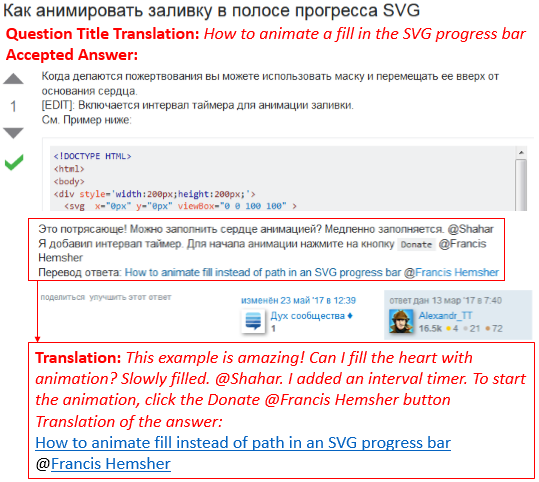
\includegraphics[width = 0.48\textwidth]{figures/exmp1.png}
		\label{fig:RSOanswerExample}}
	\hfill
	\subfigure[\#42672537: The referenced ESO question with the accepted answer]{  
		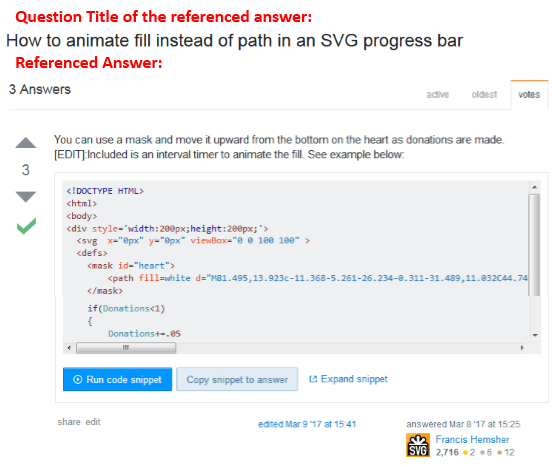
\includegraphics[width = 0.48\textwidth]{figures/exmp2.png}
		\label{fig:ESOanswerExample}
	}
	\caption{An example of manual cross-site linking and translation}
	\label{fig:linkExample}
\end{figure}

\subsection{Cross-site Retrieval}
\label{sec:crossLinking}
Since its launch in 2007, English Stack Overflow has accumulated a large pool of computer programming knowledge, including 16 million questions and 24 million answers.
In contrast, the non-English Stack Overflow sites have been launched in recent years.
As the non-English Stack Overflow users and the English Stack Overflow users do share some common interests, it is very likely that some questions asked on a new non-English Stack Overflow site may have been already asked or even answered on the English Stack Overflow.
If we can recommend relevant, high-quality questions and answers (e.g., accepted or highly-voted by the community) on English Stack Overflow to the users of the new non-English Stack Overflow site, it will benefit the new site.

There are two types of users in a multi-lingual Stack Overflow site: those speak only the native language, and those can at least read some English.
For the users who can read some English, the recommendation will lead them to the relevant posts on English Stack Overflow which directly satisfy their information needs.
For the users who speak only the native language, even though they cannot understand the English descriptions, they can at least understand some code snippets or APIs mentioned in the English posts, which are the real ``meat'' of computer programming knowledge.
Therefore, these non-English speaking users can still benefit from the recommendation of relevant English posts.

However, it is not an easy task to retrieve duplicate or related posts across multi-lingual Stack Overflow sites for two reasons.
First, there is a natural language gap between non-English Stack Overflow and English Stack Overflow.
%, considering most users' English in the non-English Stack Overflow.
Second, there are too many posts in Stack Overflow to retrieve related posts, and these post themselves often have lexical gap, i.e., they discuss the same computer programming knowledge but use very different words~\cite{chen2016learning}.
So an effective cross-site retrieval tool is needed.

Our cross-site retrieval method in the last section has the potential to be adopted for this purpose, as it can bridge both the language gap and lexical gap to certain extent.
To validate this potential, we use the 50 Russian \textit{Python} questions that have manual hyperlinks to ESO posts in Section~\ref{sec:explicitLink} as query questions to retrieve relevant ESO questions from the question database of 779,370 English \textit{Python} questions.
For 29 (58\%) of these 50 Russian \textit{Python} questions, the retrieved top-10 ESO questions by our method contain the ESO posts that RSO users manually hyperlink in the 50 Russian \textit{Python} questions.
%The results show that 29 (58\%) of the ground truth are in the top-10 recommendations.
For the rest 21 Russian questions, we further analyze the human-hyperlinked ESO posts that our method fails to retrieve in the top-10 ESO questions.
For example, the RSO question ``\foreignlanguage{russian}{Порядок удаления элементов списка в python}''\footnote{\url{https://ru.stackoverflow.com/questions/55464/}} (``the removal of elements of the list in python'') has a hyperlink to an ESO question ``Calling del on a list''\footnote{\url{https://stackoverflow.com/questions/8205102/}}.
In this example, ``del'' is a function name for deleting.
However, our method currently cannot reliably capture such domain-specific information and sentence-level semantics.

Therefore, although promising, our cross-site retrieval method still need to be enhanced, for example, replacing the current word-level semantic modelling with more advanced sentence-level semantic methods~\cite{kiros2015skip, conneau2017supervised} for better performance. 
Furthermore, our current analysis is anecdotal.
More formal evaluation should also be carried out to validate the effectiveness and efficiency of a cross-site retrieval method.

\subsection{Cross-site Translation}
\label{sec:crossTranslation}
Although cross-site retrieval across multi-lingual Q\&A sites is useful for users, it is just the first step, not the ultimate solution.
To assist non-English speaking users in fully exploiting the existing knowledge in English Stack Overflow, some English questions and answers especially those highly-viewed, highly-voted ones should be translated into other languages.
It was also mentioned in some comments on the announcement of multi-lingual Stack Overflow sites, such as ``\textit{I think a better idea would be to let the community translate each question and answer--think of it as a kind of editing capability.}'', ``\textit{...If someone finds a really good question on a site, with a good answer, they can translate it to other sites, post it on those sites (cite the original of course)...}''.

Breaking the language barrier would make the entire world more knowledgeable, and even users who cannot speak English at all can fully benefit from the knowledge on English Stack Overflow.
As translating could cost less effort than drafting an answer as good as the well-examined one on English Stack Overflow, it may save much effort of core users in the multi-lingual site who serve as the backbone for the relatively new site.

Recently, machine translation has made big progress by incorporating deep learning methods~\cite{wu2016google, sutskever2014sequence}. 
To assist high-quality translation, we can adopt the power of advanced machine translation to first obtain an overall translation, and then let human users revise the translation.
However, the general machine translation system may not work well for Q\&A discussions, and it needs to be improved in two aspects.
First, current machine translation models focus on sentence-level translation without contextual information.
However, to translate an answer well in a Q\&A discussion thread, the model not only needs to consider the current sentence in the answer, but also needs to take the corresponding question information into consideration.
Second, Stack Overflow is a domain-specific site about computer programming, while the current machine translation system is trained for general purpose.
Many domain-specific words will be out of vocabulary or have different meanings from daily life such as ``bug'', ``port'', etc.
So the general machine translation model must be customised by incorporating the domain-specific knowledge.

In addition to technical aspect of cross-site translation, we also need to design some mechanisms to motivate users to contribute to the translation activity.
We can set up a reward rule that once users translate one answer from English Stack Overflow to non-English site, they can earn some award points.
Once other users vote their translated answer, they will earn more points and reputation score.
A translator badge can also be created and awarded to users whose translation score reaches to a certain level.

\begin{comment}
\subsection{Guideline to other Q\&A sites}
\textcolor{red}{CCY: Maybe we talk about how our discovery in Stack Overflow can help guide the development of multilingual variants to other similar Q\&A sites. Or we may talk about the similar situation of Quora.}

\textcolor{blue}{I think this belongs to here.
	There are three types of programmers in the world: 
	1) Those who are comfortable participating on a site in English. They won't be affected by the existence of SO in other languages. 
	2) Those who can read English but not express themselves. Most developers can understand some English as the most programming languages are written in English. But being able to understand what a few select words (i.e., as a programmer) does not necessarily mean being proficient enough in a language to read or write. Therefore, some developers even though can read and write English without any problems prefer to ask or answer questions in their native language. Let's bring Yukihiro Matsumoto\footnote{\url{https://en.wikipedia.org/wiki/Yukihiro_Matsumoto}} (also known as Matz, he's the inventor of Ruby, one of the most popular programming languages in the world) and Ruby as an example. Matz knows English and has given several talks in English but yet he still got his programming blog in Japanese. And at the beginning of Ruby, most of its documents are also in Japanese. They can benefit from Stack Overflow, but they can't contribute. 
	3) Those who can't speak English at all. They can't even benefit from Stack Overflow.
	According to our empirical study in this section, creating SO sites in other languages does attract programmers of type 2. 
	But they weren't contributing much to Stack Overflow in the first place, so Stack Overflow isn't losing too much by it.
}
\end{comment}

\begin{comment}
\textcolor{red}{Some quotes from users' comments.}
I think a better idea would be to let the community translate each question and answer--think of it as a kind of editing capability. 
You don't need a formal system in place to do that. If someone finds a really good question on a site, with a good answer, they can translate it to other sites, post it on those sites (cite the original of course) and then, if other users find it valuable, they can then vote on the translated version. If the content is not useful, they don't get rep, if it is, they do, based on votes. This would encourage the translation of the quality content, and discourage the translation of the crap.
But a GREAT IMPROVEMENT would be creating an auto-translate system to all Stack Exchange websites, which means: any text that is not inside a `code` block would be viewed in the user's language. It'd be great mainly because currently a lot of good questions/answers are only known to a particular language, so breaking the language barrier would make the entire world more knowledgeable. The option to view it in the original language or use other translation engines (provided externally, fecthing through Javascript) would be a plus. Anyway, congratulations in joining Portuguese and Japanese in the seemly growing Stack Overflow languages websites group :)
Maybe a good idea would be to award points to users willing to translate answers from the english version into portuguese; a translator badge could be created even. My one bit of criticism is that my reputation from stackoverflow didn't move over to the portuguese version. I kinda expected that.
This is the world wide web and it is built on a thing called hypertext. Multiple languages? Cool, that's the "world" part. But don't forget about hypertext. Please, make sure that questions and answers can be linked easily across the different language sites. If someone asks a question in Japanese that is essentially a duplicate of an existing English question, linking the two questions will allow Japanese speakers (who might understand *some* English, or at least be able to read code snippets) to get immediate value from past answers, without waiting for new answers and without waiting for translation. Although such links would also aid translators.
This could be the first step towards a multilingual stack exchange. Where every site is available in every language. There shouldn't be a language version of stackoverflow, instead stackoverflow should have built in support for different languages and a workflow for translating into all of those languages. With the help of translation, both machine and human, the knowledge that non English speakers have can be shared with English speakers and vice versa.	
\end{comment}

	\section{Conclusion and Future Work}

In this paper, we carry out an empirical study to explore the evidences in favor of or against multi-lingual Q\&A sites.
Our study examines not only the user perspective, including user registration, posting behavior and reputation score, but also the knowledge perspective, including tag uniqueness and tag correlation between multi-lingual sites, and explicit cross-site links created by users and implicit cross-site links that users are not aware of.
Our study results help to resolve the arguments about the risk of community split and the knowledge needs and interests in non-English language.
We also confirm the validity of the concern about knowledge fragmentation and duplication, and provide a promising cross-site retrieval method for mitigating this issue.

Our evidence-based study method provides a guideline to study the pros and cons of multi-lingual Q\&A sites, and our findings shed the light on the development of multi-lingual Q\&A sites.
In the future, based on our findings, we will develop tools to help bridge the gap across multi-lingual Q\&A sites, such as recommending duplicate or related posts on English Stack Overflow to Russian Stack Overflow questions, and developing domain-specific deep learning based machine translation model for Q\&A discussions.

\begin{comment}
show the influence of the launch of multi-lingual Stack Overflow.
We first spot the fierce debate of the decision of building multi-lingual Stack Overflow, and obtain the pros and cons by analysing users' comments under the announcement of the new sites.
To validate the benefits and concerns, we carry out quantitative empirical study between English Stack Overflow and Russian Stack Overflow from both user and content aspects.
The results show the value of existence of multi-lingual Stack Overflow and resolve some concerns like community split of the main site.
Some concerns are also confirmed such as knowledge fragmentation and content duplication.
These discoveries can play an important criteria to guide the future development of not only multi-lingual Stack Overflow, but also other Q\&A sites like Quora.
\end{comment}



\par

%Last but not least, we will implement a new recommending tool that will be deployed on Stack Overflow or some other Q\&A websites to assist non-English language speakers to utilize the knowledge in the English Q\&A site better.
	
	\bibliographystyle{ACM-Reference-Format}
    \bibliography{reference}	

	
	% that's all folks
\end{document}


